\section{Fragmentos originales}
\subsection{Fragmento 1}
\label{frag1eng}
\begin{quotation}
    \emph{``news articles that are intentionally and verifiably false, and could mislead readers''} --- \hyperref[frag1esp]{Fragmento en castellano}
\end{quotation}

\subsection{Fragmento 2}
\label{frag2eng}
\begin{quotation}
    \emph{``fabricated information that mimics news media content in form but not in organisational process or intent''} --- \hyperref[frag2esp]{Fragmento en castellano}
\end{quotation}

\subsection{Fragmento 3}
\label{frag3eng}
\begin{quotation}
    \emph{``fake news appropriates the look and feel of real news; from how websites look; to how articles are written; to how photos include attributions. Fake news hides under a veneer of legitimacy as it takes on some form of credibility by trying to appear like real news. Furthermore, going beyond the simple appearance of a news item, through the use of news bots, fake news imitates news’ omnipresence by building a network of fake sites.''} --- \hyperref[frag3esp]{Fragmento en castellano}
\end{quotation}

\subsection{Fragmento 4}
\label{frag4eng}
\begin{quotation}
    \emph{``Information is propositional content in that it proposes that a specific state of the world exists: it is `what must be the case in the world for the sign to exist as and when it does'.''} --- \hyperref[frag4esp]{Fragmento en castellano}
\end{quotation}

\subsection{Fragmento 5}
\label{frag5eng}
\begin{quotation}
    \emph{``\underline{Misinformation.} Propositional content of signs that misrepresents the state of the world without the intention to deceive [...]. One area where this [...] is quite common is health advice in online communities \citep{Venkatesan2014}, where many people spread false information unintentionally \citep{Myers2009}.''}  --- \hyperref[frag5esp]{Fragmento en castellano}
\end{quotation}

\subsection{Fragmento 6}
\label{frag6eng}
\begin{quotation}
    \emph{``\underline{Disinformation.} Propositional content of signs that misrepresents the state of the world with the intention to deceive.''}  --- \hyperref[frag6esp]{Fragmento en castellano}
\end{quotation}

\subsection{Fragmento 7}
\label{frag7eng}
\begin{quotation}
    \emph{``\underline{Malinformation.} Propositional content of signs that truthfully represents the state of the world with the intention to deceive [...] It is often assumed that deception appears in the form of or as result of bald-face lying and other forms of disinformation. However, deception can equally happen in the form or as a result of subtle manipulation of information that does not necessarily misrepresent the world but is intended to deceive \citep{McCornack2009,McCornack2014,Wardle2018a}. Examples include half-truths and spin, which refer to incomplete or selective information provided with the intention to deceive \citep{Fallis2016}.''} --- \hyperref[frag7esp]{Fragmento en castellano}
\end{quotation}

\clearpage
\section{Visualización SHAP}

\subsection{Politifact-Snopes One Evidence}
\label{fig:shap-ps-one-annex}

\begin{figure}[!ht]
    \captionsetup[subfigure]{justification=Centering}
    % BERT BASE (UNCASED / CASED)
    \begin{subfigure}[t]{0.4\textwidth}
        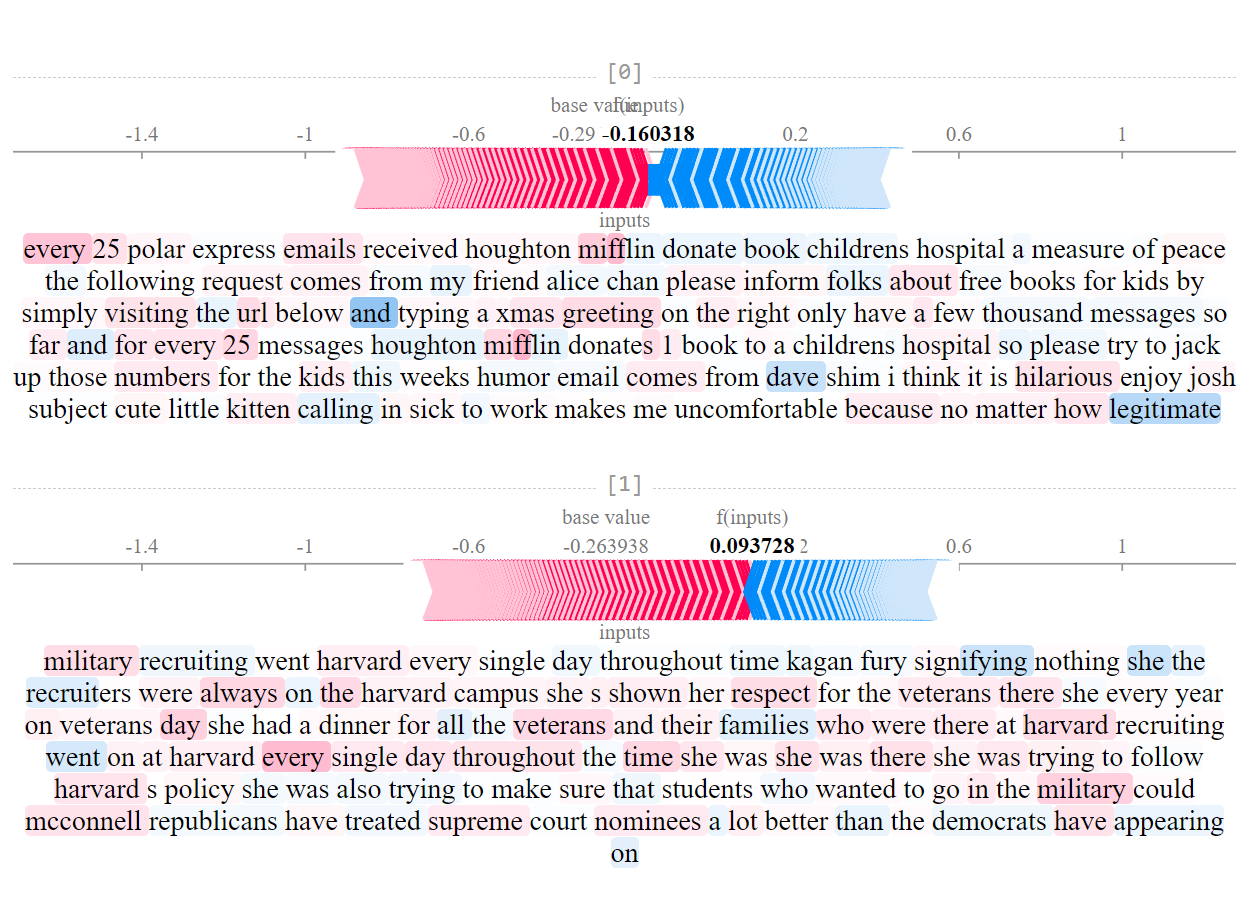
\includegraphics[width=\textwidth]{figs/one_TF/bert-b-u.png}
        \caption{{BERT}\textsubscript{B, U}}
    \end{subfigure}
    \hspace{\fill} % maximize horizontal separation
    \begin{subfigure}[t]{0.4\textwidth}
        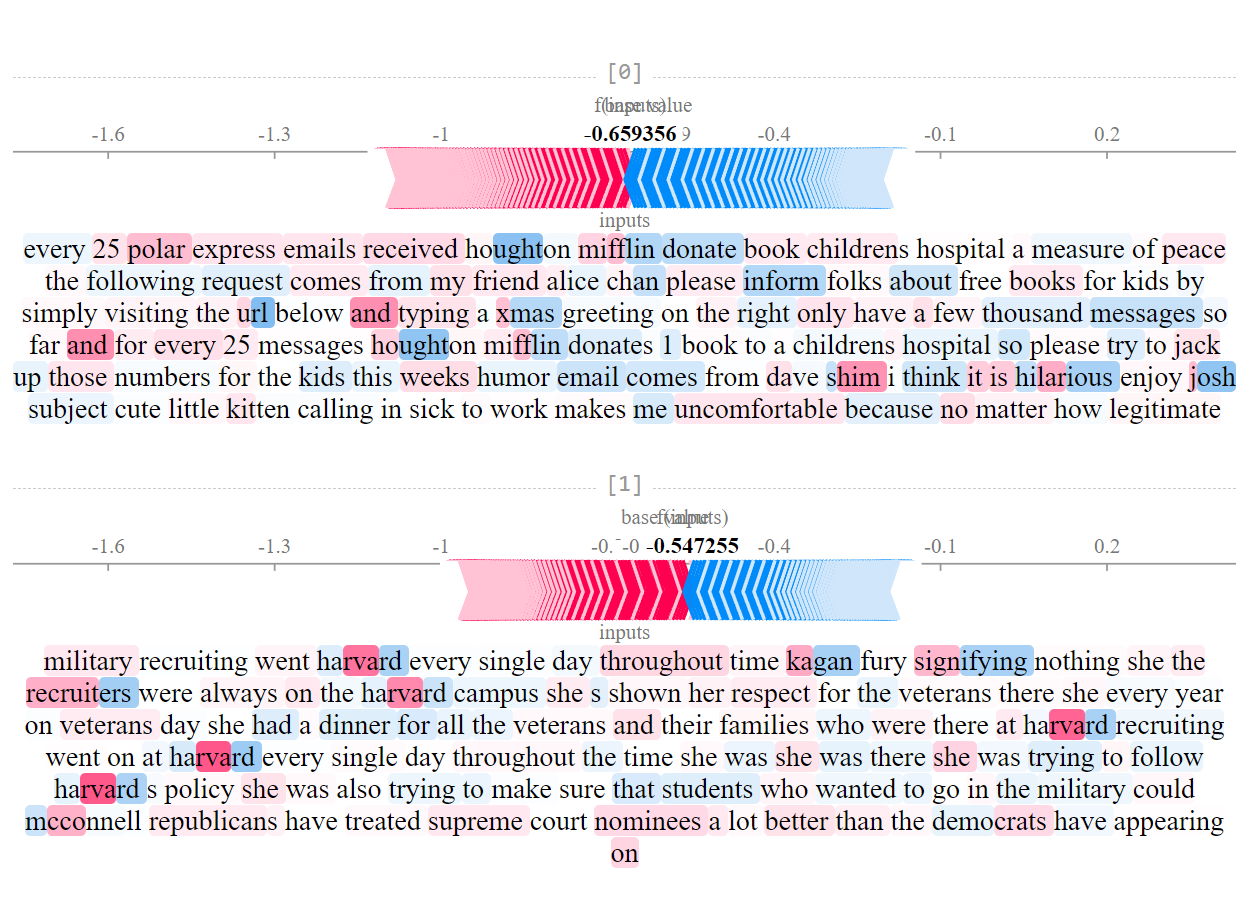
\includegraphics[width=\linewidth]{figs/one_TF/bert-b-c.png}
        \caption{{BERT}\textsubscript{B, C}}
    \end{subfigure}


% \end{figure}
% \begin{figure}[h]\ContinuedFloat
%     \captionsetup[subfigure]{justification=Centering}

    % BERT BASE MULTILINGUAL (UNCASED / CASED)
    \begin{subfigure}[t]{0.4\textwidth}
        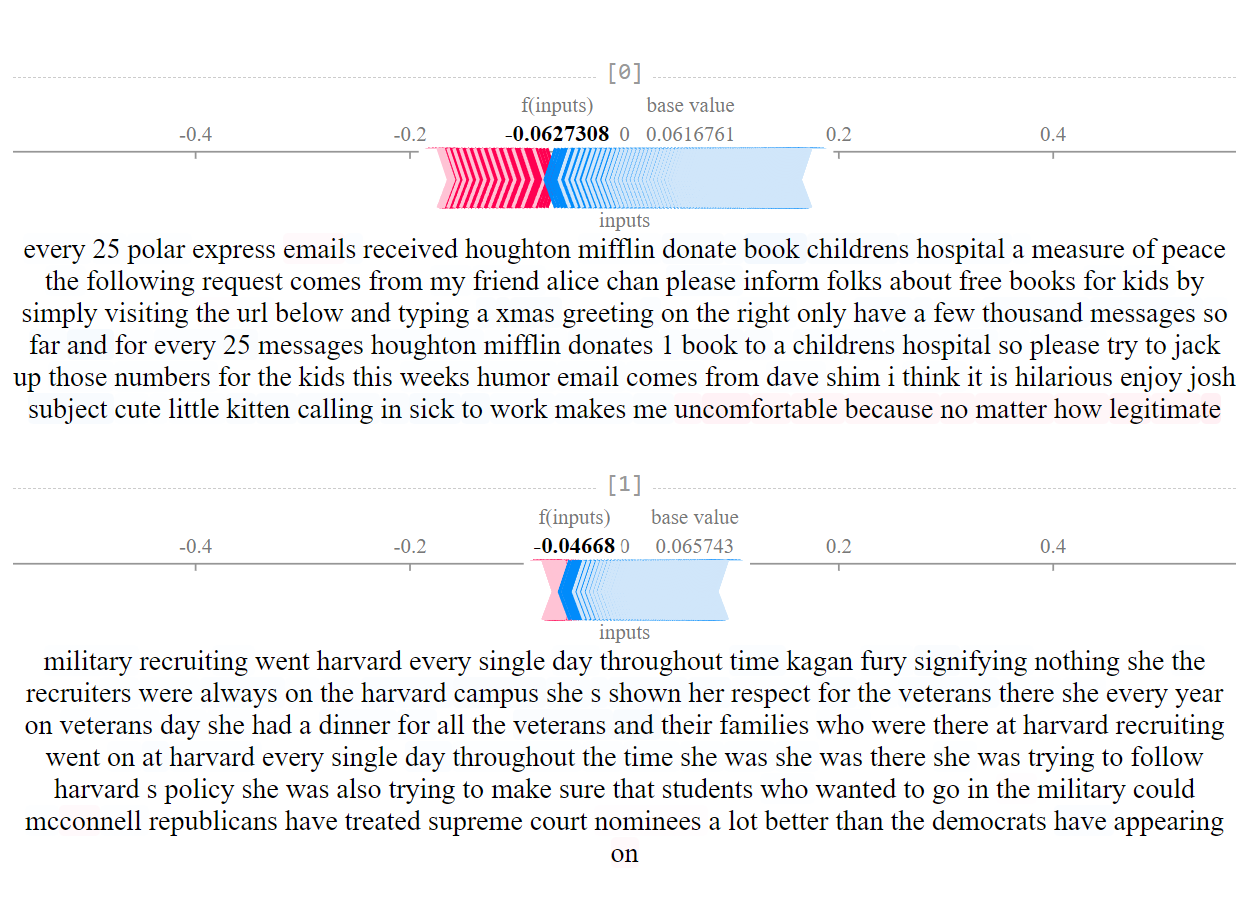
\includegraphics[width=\textwidth]{figs/one_TF/bert-b-ml-u.png}
        \caption{{BERT}\textsubscript{B, U, ML}}
    \end{subfigure}
    \hspace{\fill} % maximize horizontal separation
    \begin{subfigure}[t]{0.4\textwidth}
        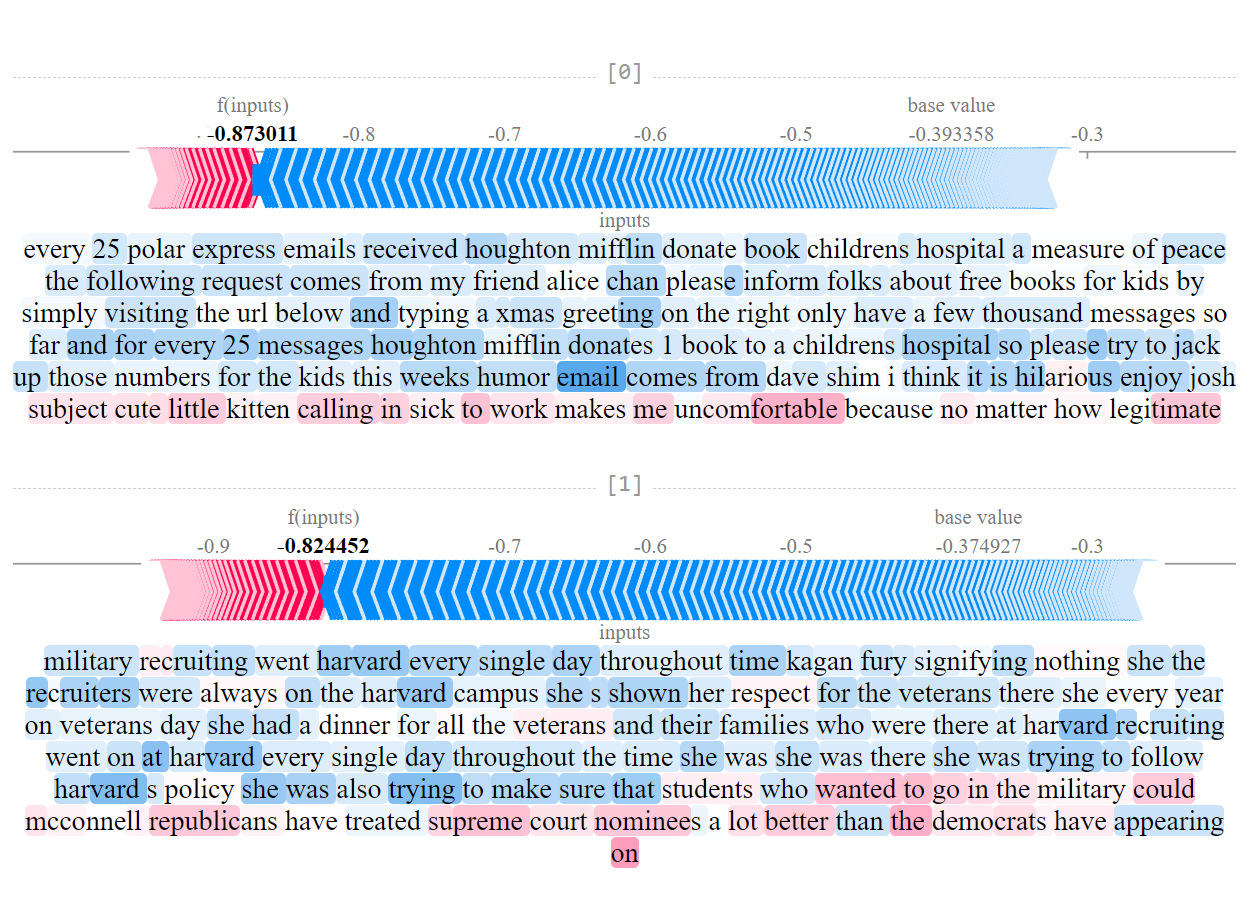
\includegraphics[width=\linewidth]{figs/one_TF/bert-b-ml-c.png}
        \caption{{BERT}\textsubscript{B, C, ML}}
    \end{subfigure}


% \end{figure}
% \begin{figure}[h]\ContinuedFloat
%     \captionsetup[subfigure]{justification=Centering}

    % BERT LARGE (UNCASED / CASED)
    \begin{subfigure}[t]{0.4\textwidth}
        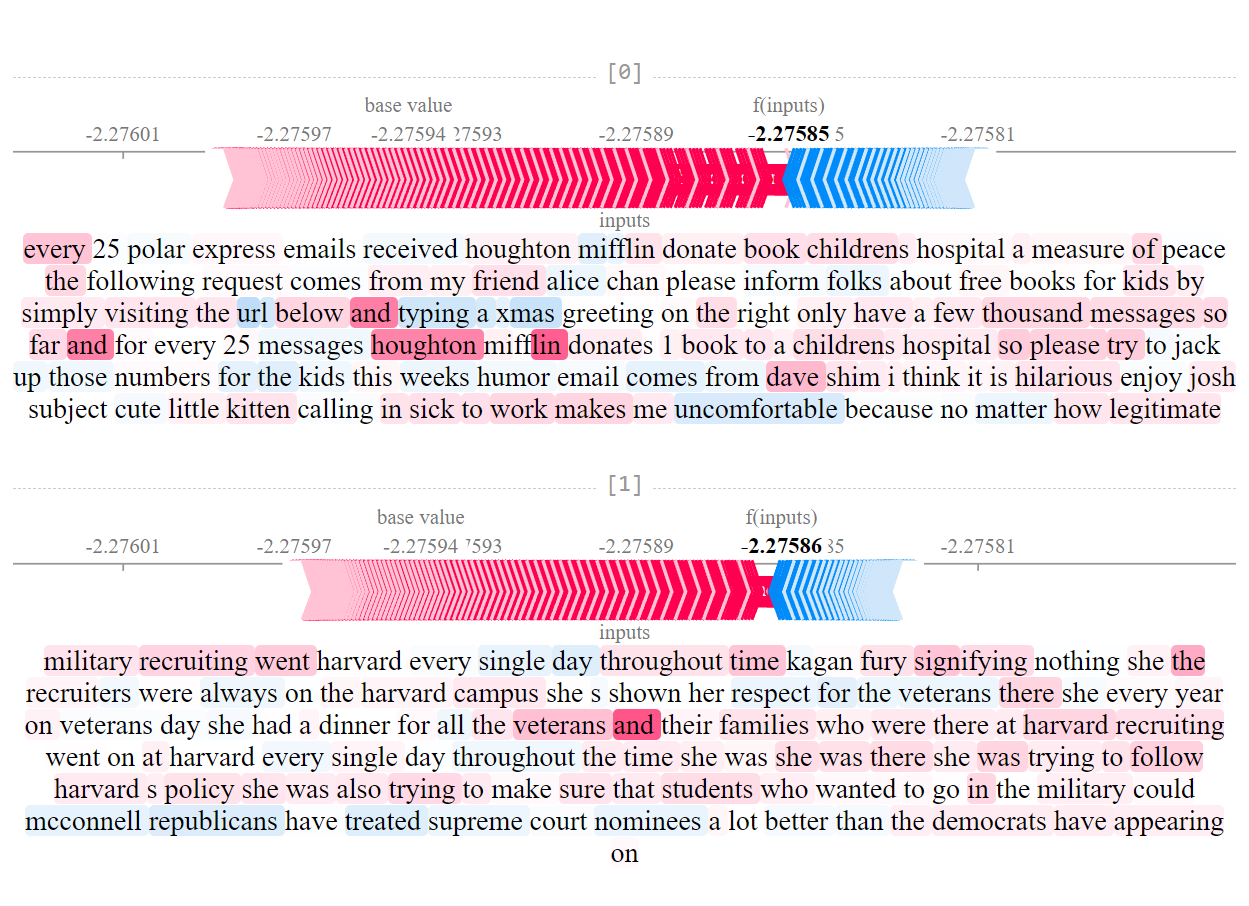
\includegraphics[width=\textwidth]{figs/one_TF/bert-l-u.png}
        \caption{{BERT}\textsubscript{L, U}}
    \end{subfigure}
    \hspace{\fill} % maximize horizontal separation
    \begin{subfigure}[t]{0.4\textwidth}
        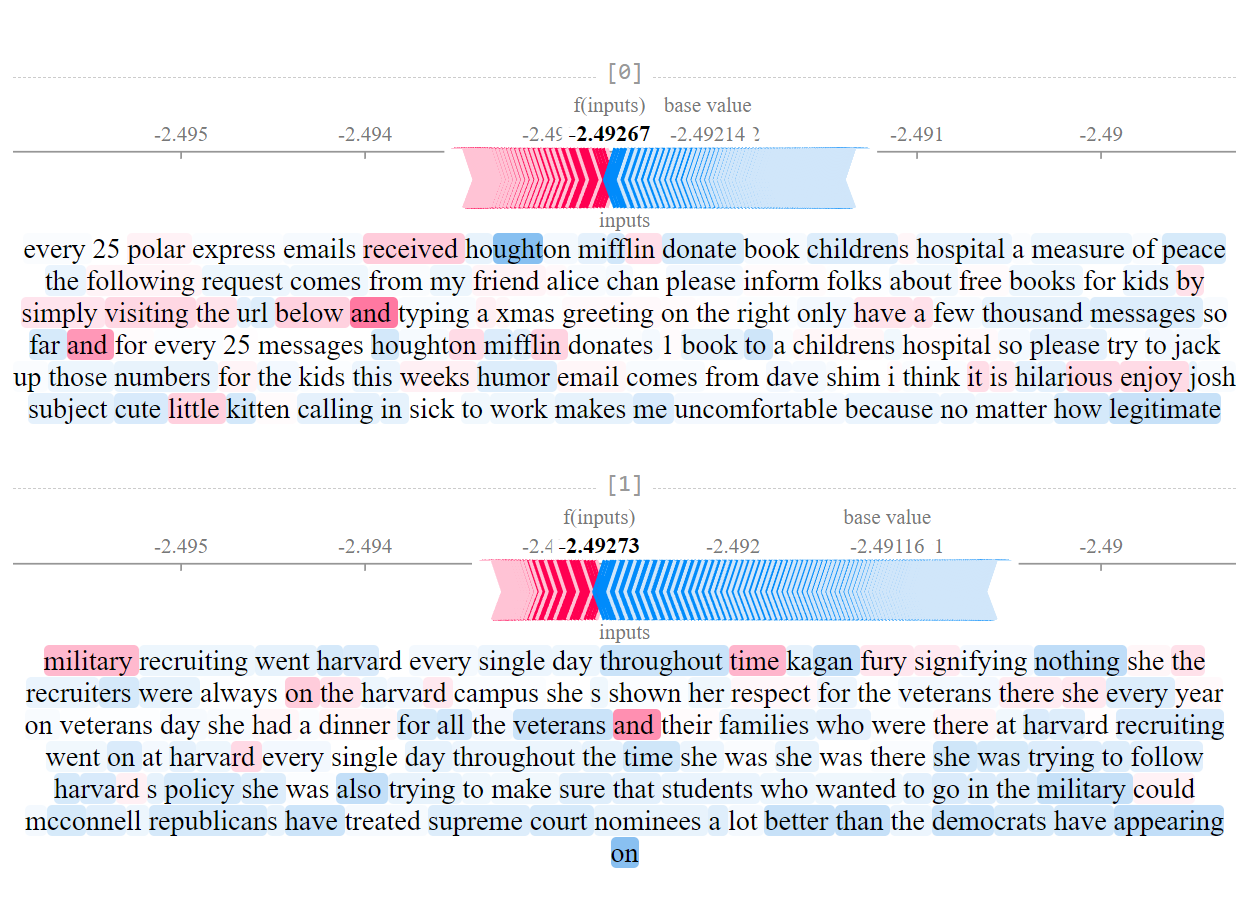
\includegraphics[width=\linewidth]{figs/one_TF/bert-l-c.png}
        \caption{{BERT}\textsubscript{L, C}}
    \end{subfigure}


% \end{figure}
% \begin{figure}[!ht]\ContinuedFloat
%     \captionsetup[subfigure]{justification=Centering}

    % DistilBERT BASE (CASED / CASED MULTILINGUAL)
    \begin{subfigure}[t]{0.4\textwidth}
        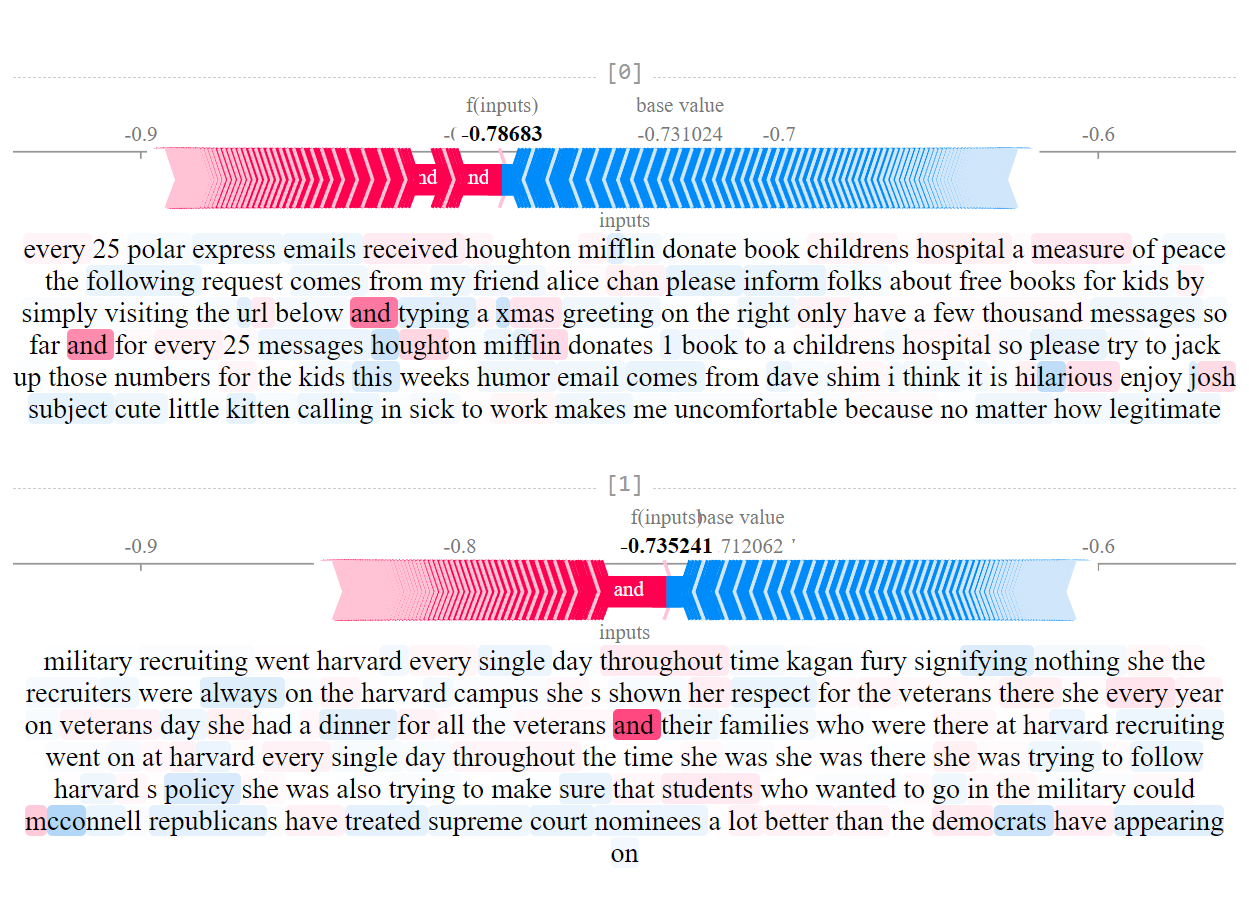
\includegraphics[width=\textwidth]{figs/one_TF/distil-b-c.png}
        \caption{{DistilBERT}\textsubscript{B, C}}
    \end{subfigure}
    \hspace{\fill} % maximize horizontal separation
    \begin{subfigure}[t]{0.4\textwidth}
        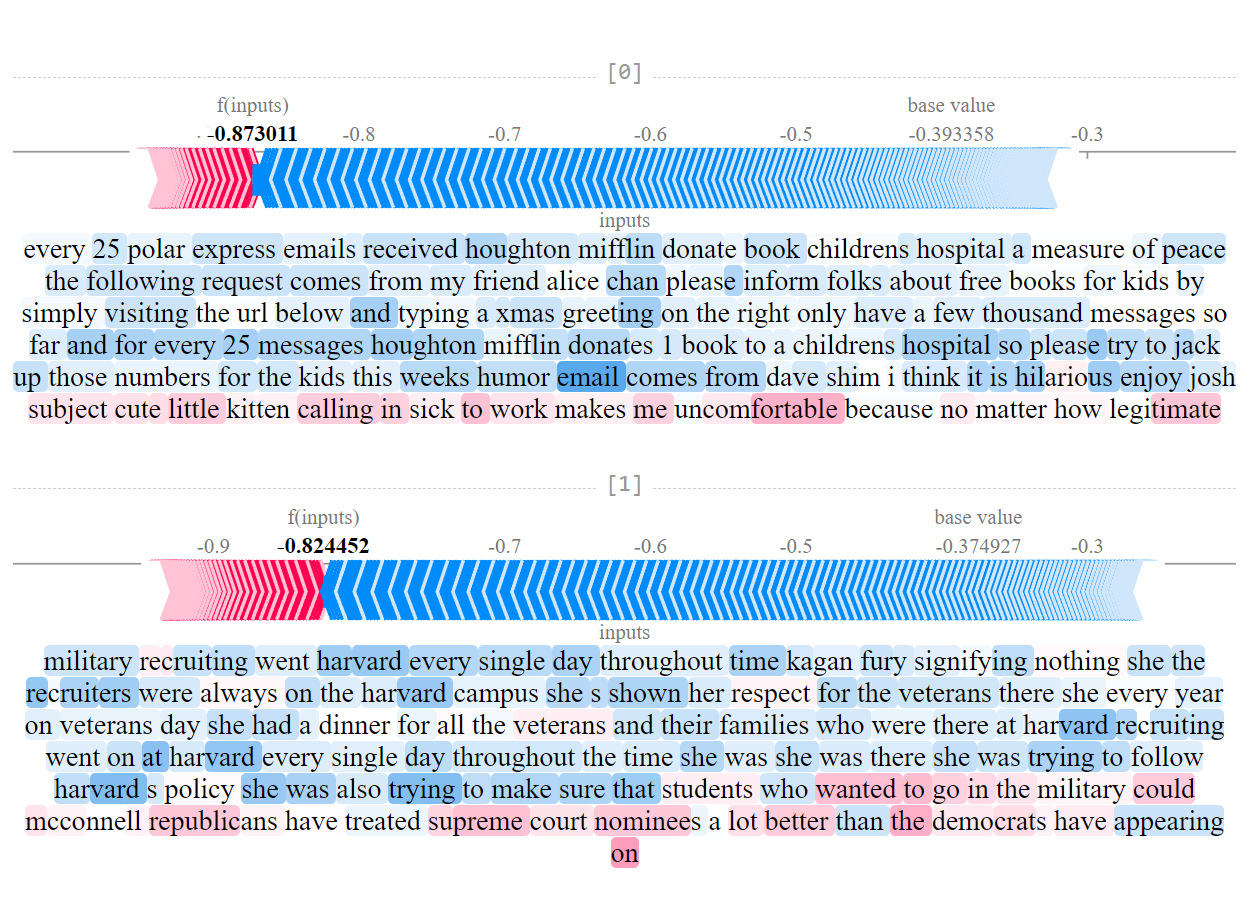
\includegraphics[width=\linewidth]{figs/one_TF/bert-b-ml-c.png}
        \caption{{DistilBERT}\textsubscript{B, C, ML}}
    \end{subfigure}


\end{figure}
\begin{figure}[!h]\ContinuedFloat
    \captionsetup[subfigure]{justification=Centering}

    % RoBERTa (BASE / LARGE)
    \begin{subfigure}[t]{0.4\textwidth}
        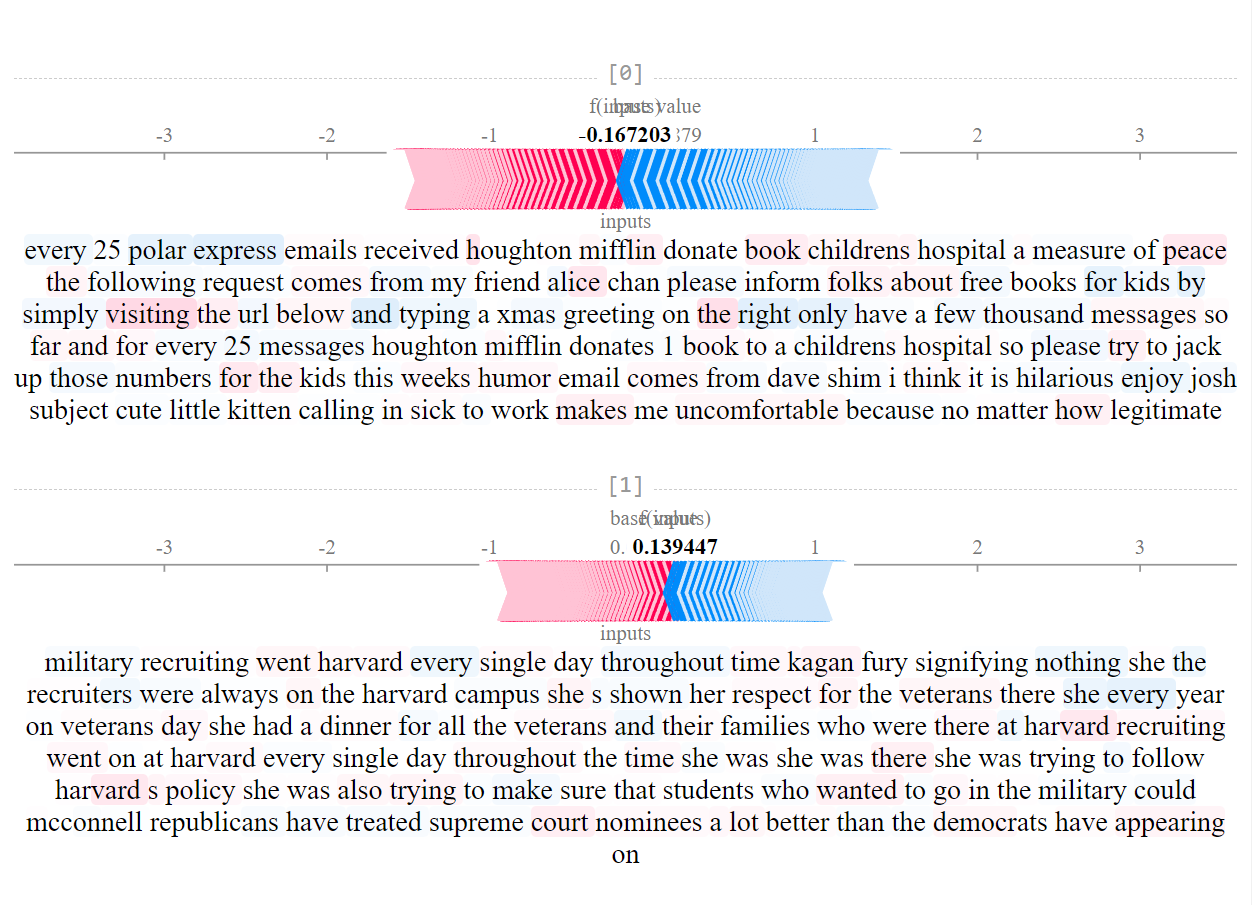
\includegraphics[width=\textwidth]{figs/one_TF/roberta-b.png}
        \caption{{RoBERTa}\textsubscript{B}}
    \end{subfigure}
    \hspace{\fill} % maximize horizontal separation
    \begin{subfigure}[t]{0.4\textwidth}
        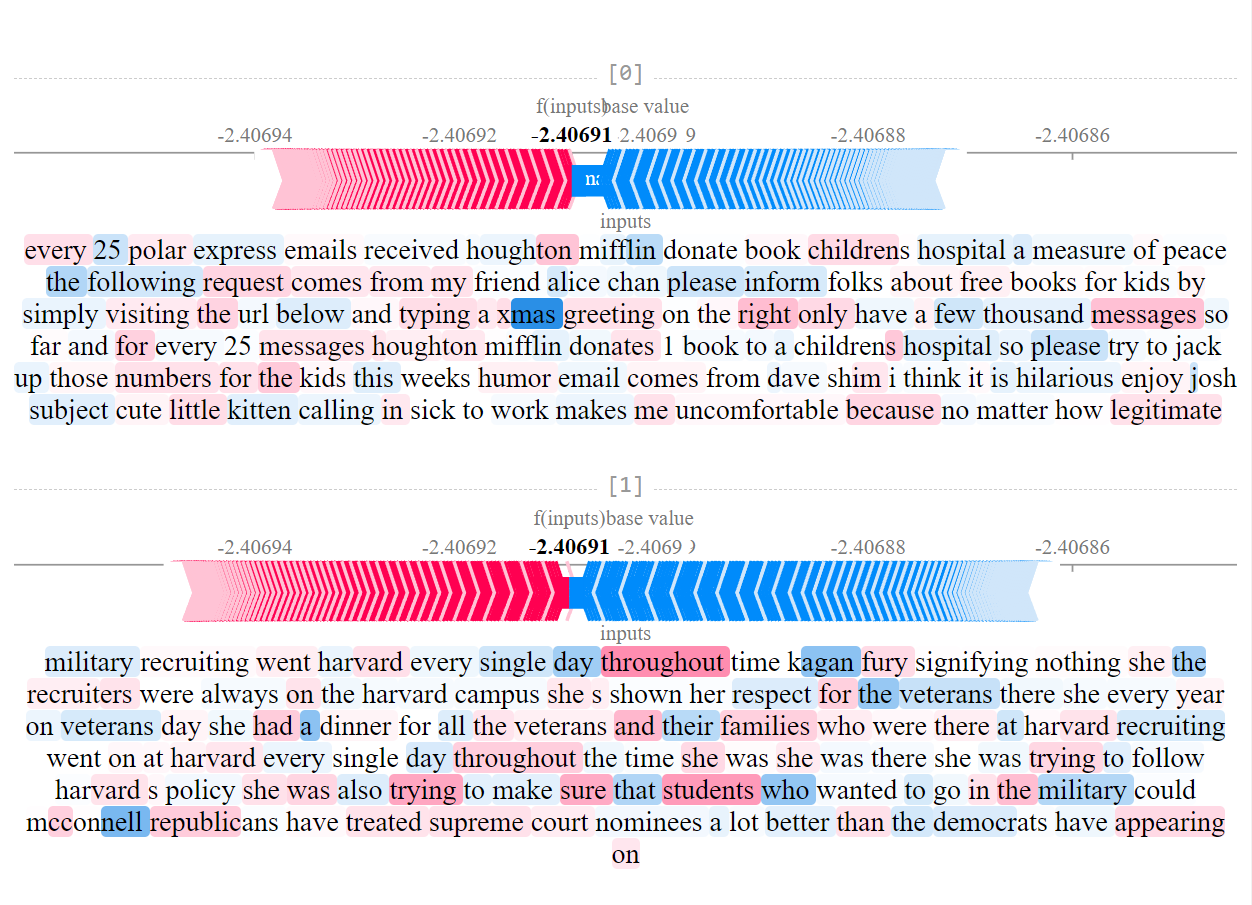
\includegraphics[width=\linewidth]{figs/one_TF/roberta-l.png}
        \caption{{RoBERTa}\textsubscript{L}}
    \end{subfigure}


% \end{figure}
% \begin{figure}[h]\ContinuedFloat
%     \captionsetup[subfigure]{justification=Centering}

    % DeBERTa (BASE / LARGE)
    % \bigskip % more vertical separation
    \begin{subfigure}[t]{0.4\textwidth}
        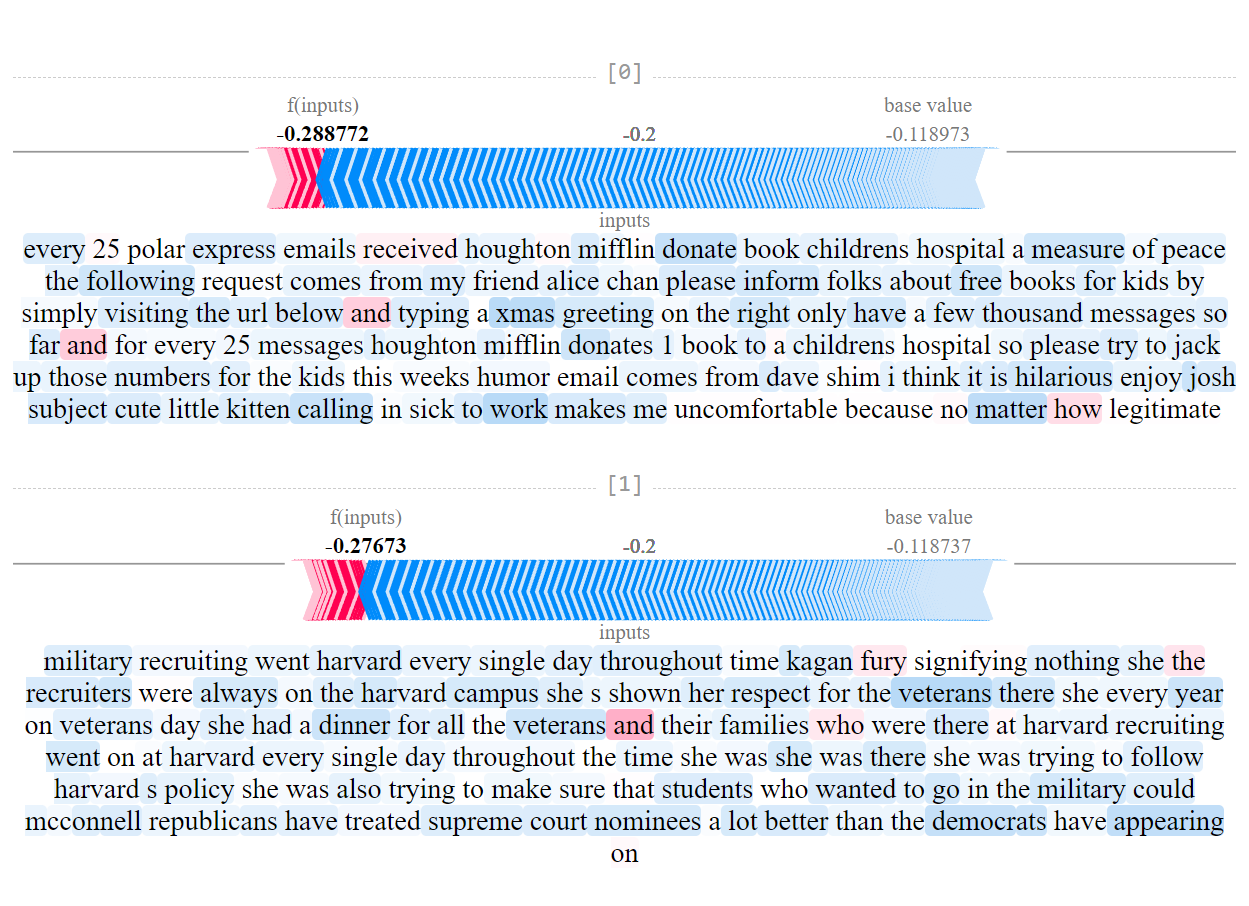
\includegraphics[width=\textwidth]{figs/one_TF/deberta-b.png}
        \caption{{DeBERTa}\textsubscript{B}}
    \end{subfigure}
    \hspace{\fill} % maximize horizontal separation
    \begin{subfigure}[t]{0.4\textwidth}
        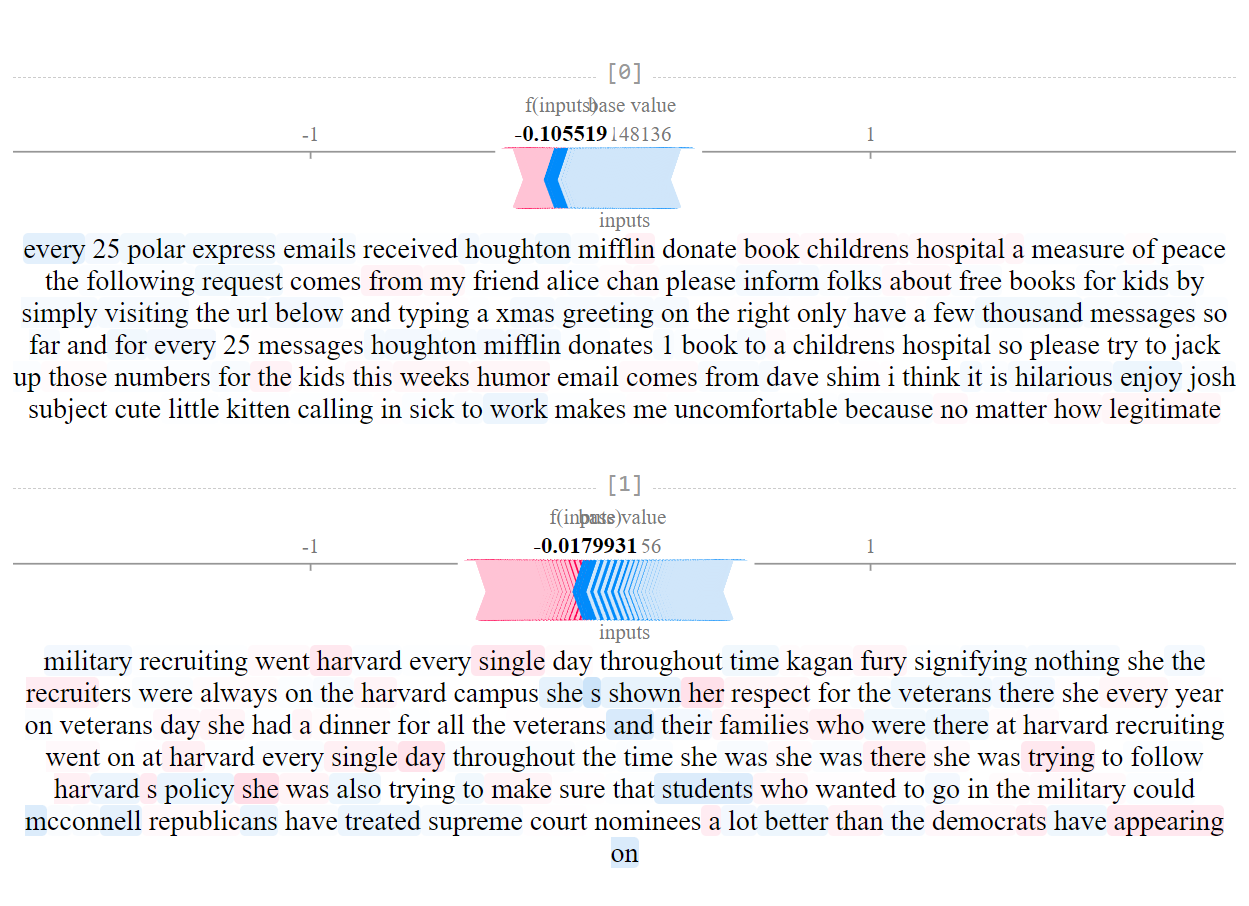
\includegraphics[width=\linewidth]{figs/one_TF/deberta-l.png}
        \caption{{DeBERTa}\textsubscript{L}}
    \end{subfigure}    
    
    \caption{Valores Shapley de cada modelo. Los subíndices utilizados para cada modelo $M$ indican respectivamente $M_{\text{B}}$: BASE; $M_{\text{L}}$: LARGE; $M_{C}$: CASED; $M_{\text{U}}$: UNCASED; $M_{\text{ML}}$: MULTILINGUAL.}
\end{figure}



\clearpage
\subsection{Politifact-Snopes All Evidences}
\label{fig:shap-ps-all-annex}

\begin{figure}[!h]
    \captionsetup[subfigure]{justification=Centering}
    % BERT BASE (UNCASED / CASED)
    \begin{subfigure}[t]{0.4\textwidth}
        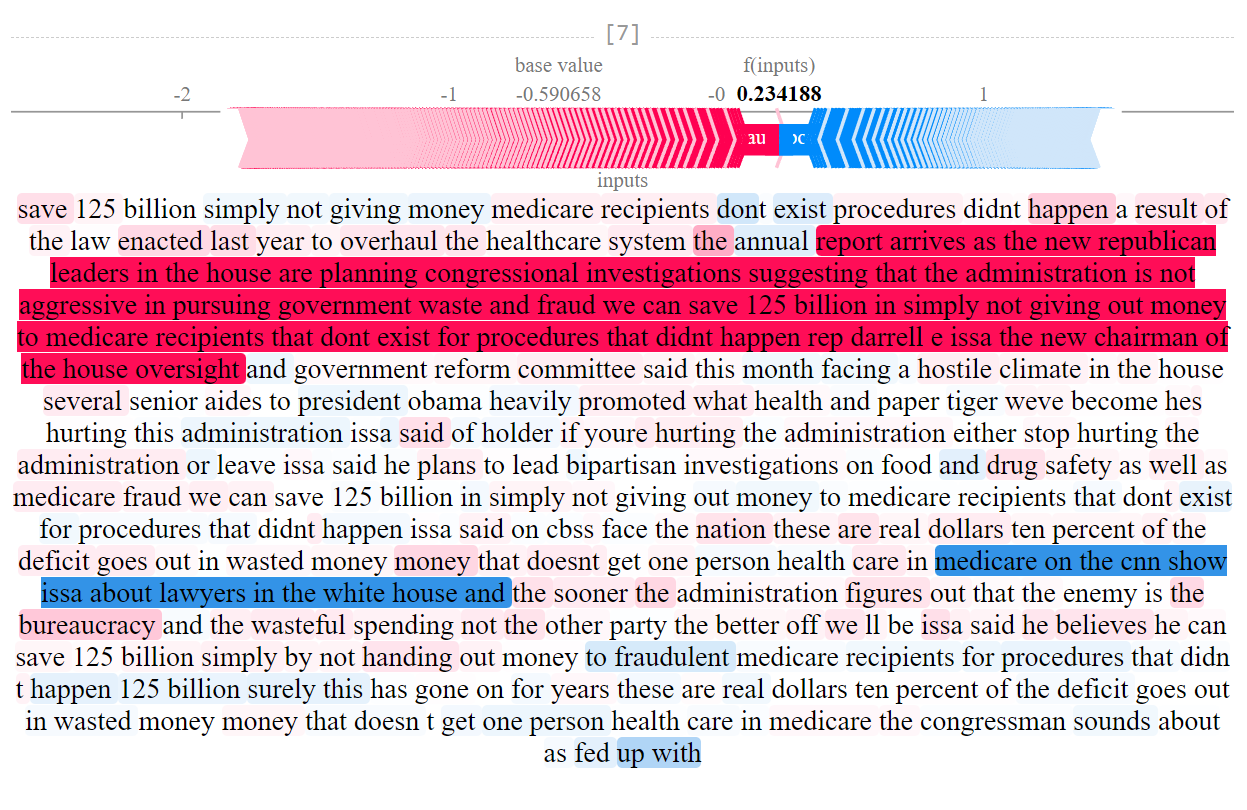
\includegraphics[width=\textwidth]{figs/all_F/bert-b-u.png}
        \caption{{BERT}\textsubscript{B, U}}
    \end{subfigure}
    \hspace{\fill} % maximize horizontal separation
    \begin{subfigure}[t]{0.4\textwidth}
        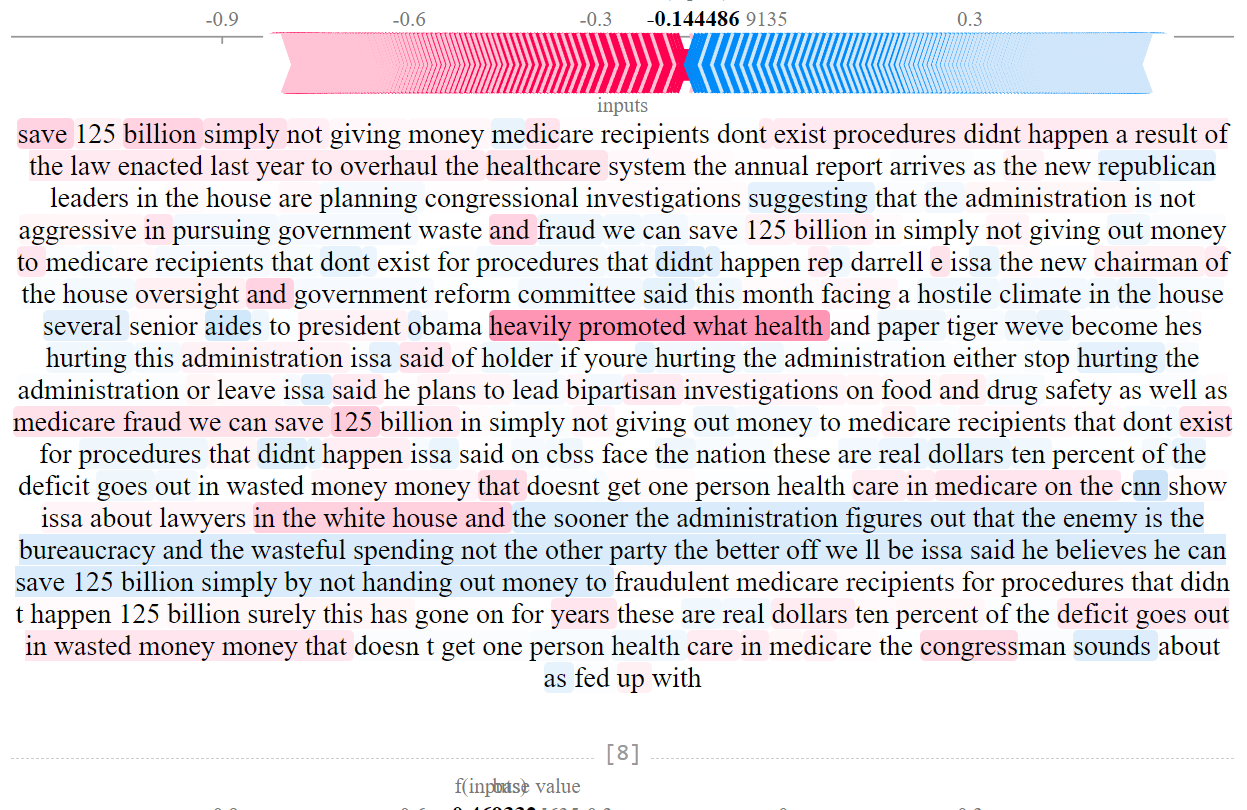
\includegraphics[width=\linewidth]{figs/all_F/bert-b-c.png}
        \caption{{BERT}\textsubscript{B, C}}
    \end{subfigure}


% \end{figure}
% \begin{figure}[h]\ContinuedFloat
%     \captionsetup[subfigure]{justification=Centering}

    % BERT BASE MULTILINGUAL (UNCASED / CASED)
    \begin{subfigure}[t]{0.4\textwidth}
        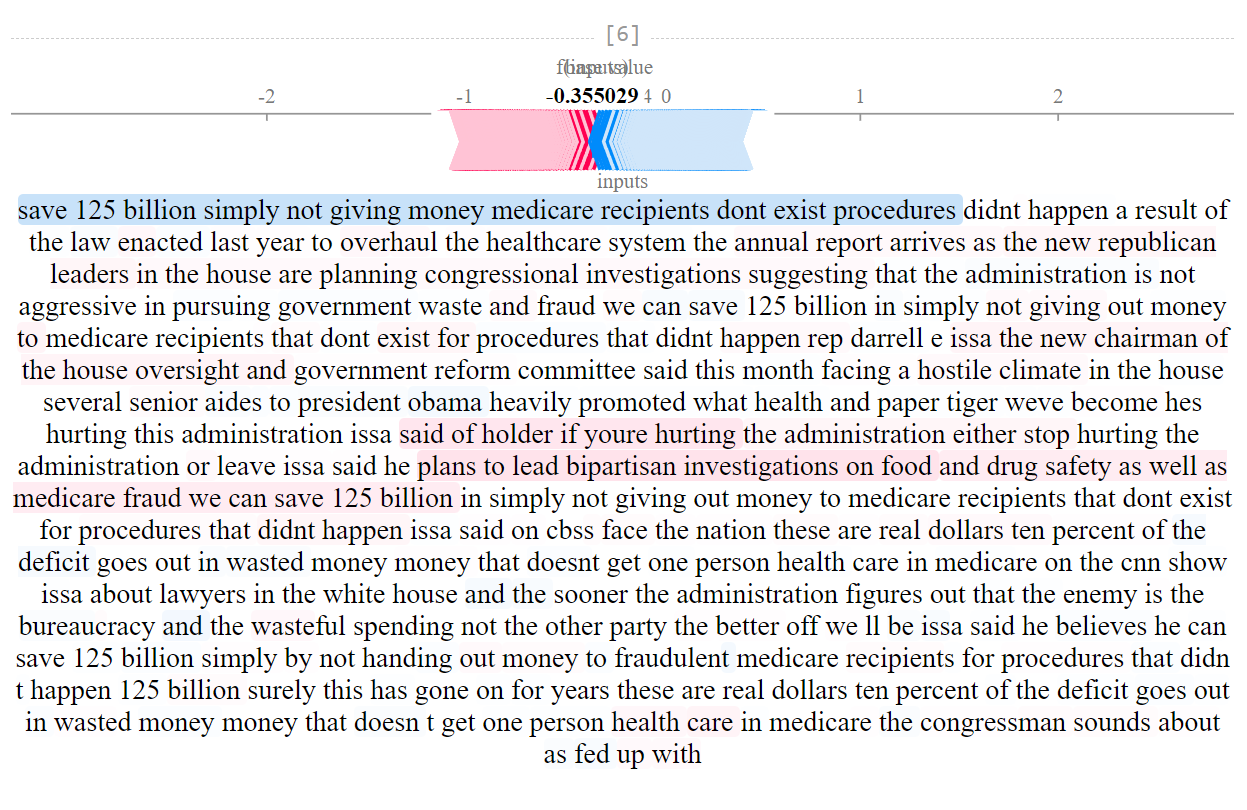
\includegraphics[width=\textwidth]{figs/all_F/bert-b-ml-u.png}
        \caption{{BERT}\textsubscript{B, U, ML}}
    \end{subfigure}
    \hspace{\fill} % maximize horizontal separation
    \begin{subfigure}[t]{0.4\textwidth}
        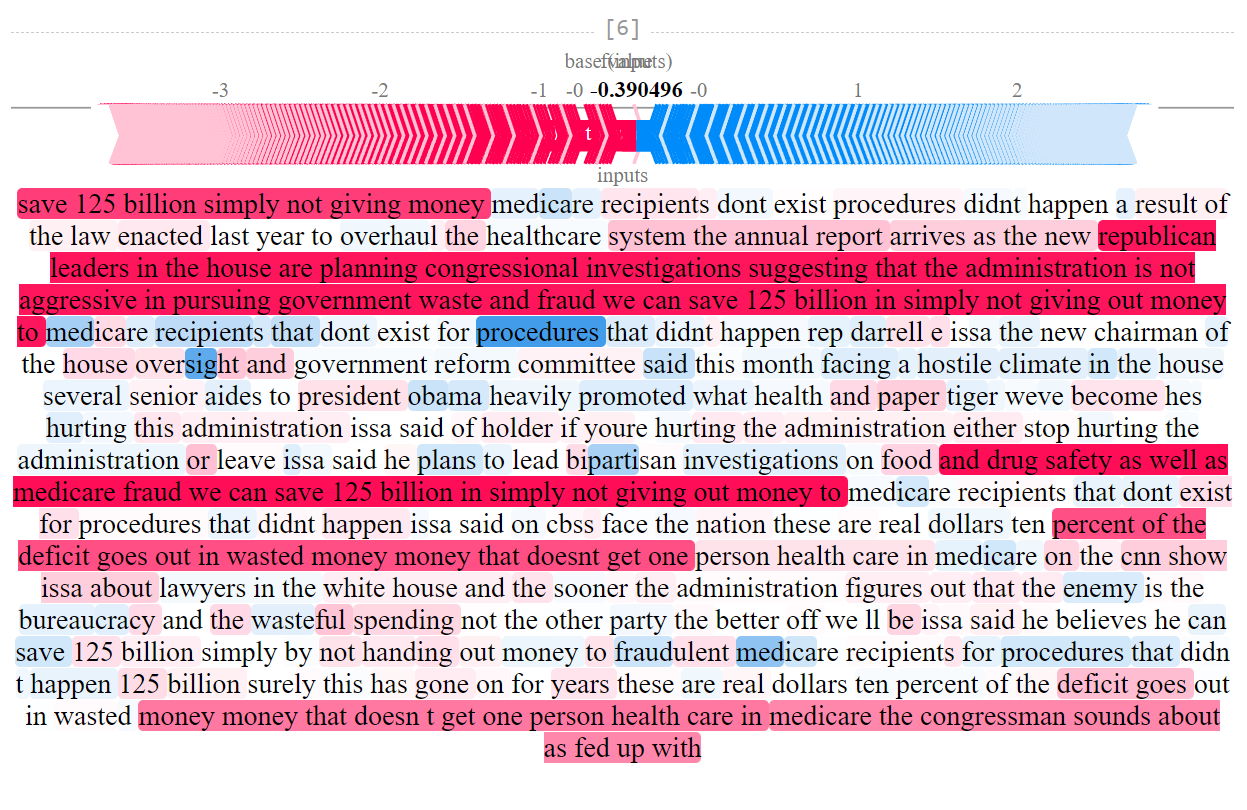
\includegraphics[width=\linewidth]{figs/all_F/bert-b-ml-c.png}
        \caption{{BERT}\textsubscript{B, C, ML}}
    \end{subfigure}


% \end{figure}
% \begin{figure}[h]\ContinuedFloat
%     \captionsetup[subfigure]{justification=Centering}

    % BERT LARGE (UNCASED / CASED)
    \begin{subfigure}[t]{0.4\textwidth}
        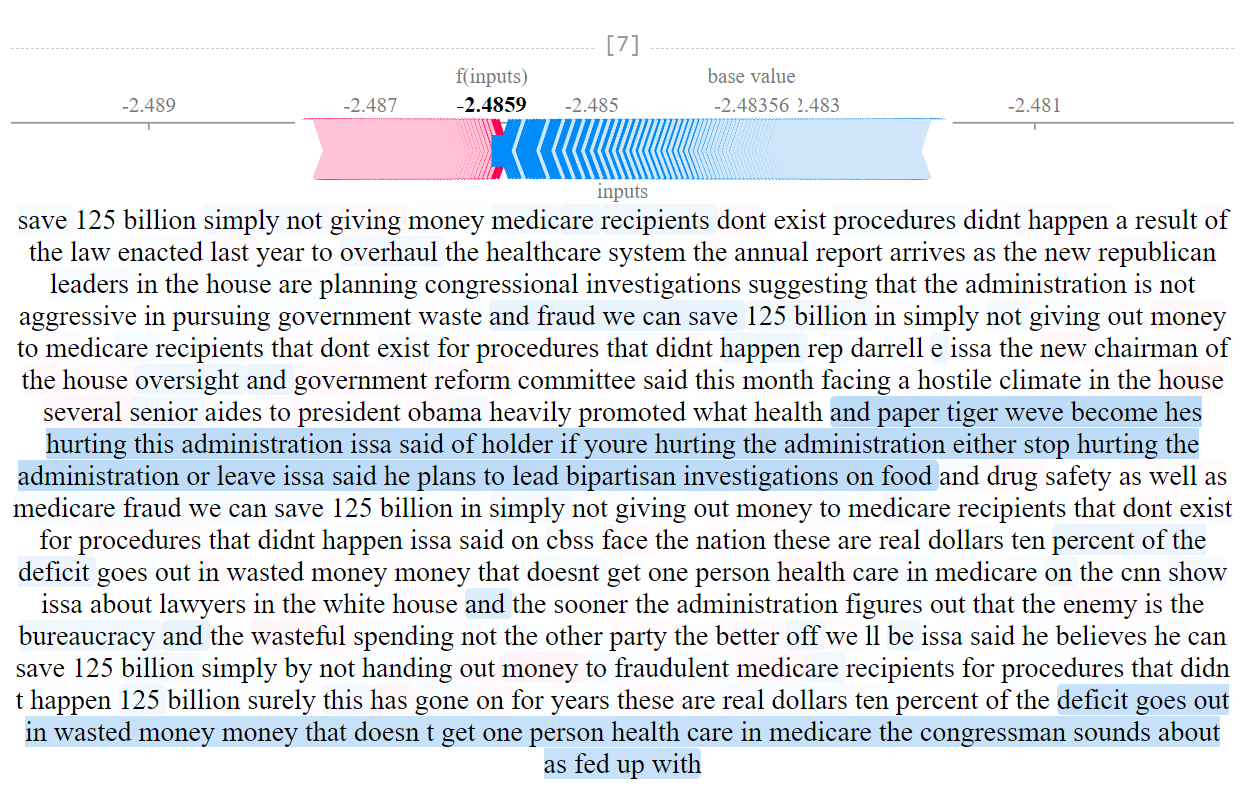
\includegraphics[width=\textwidth]{figs/all_F/bert-l-u.png}
        \caption{{BERT}\textsubscript{L, U}}
    \end{subfigure}
    \hspace{\fill} % maximize horizontal separation
    \begin{subfigure}[t]{0.4\textwidth}
        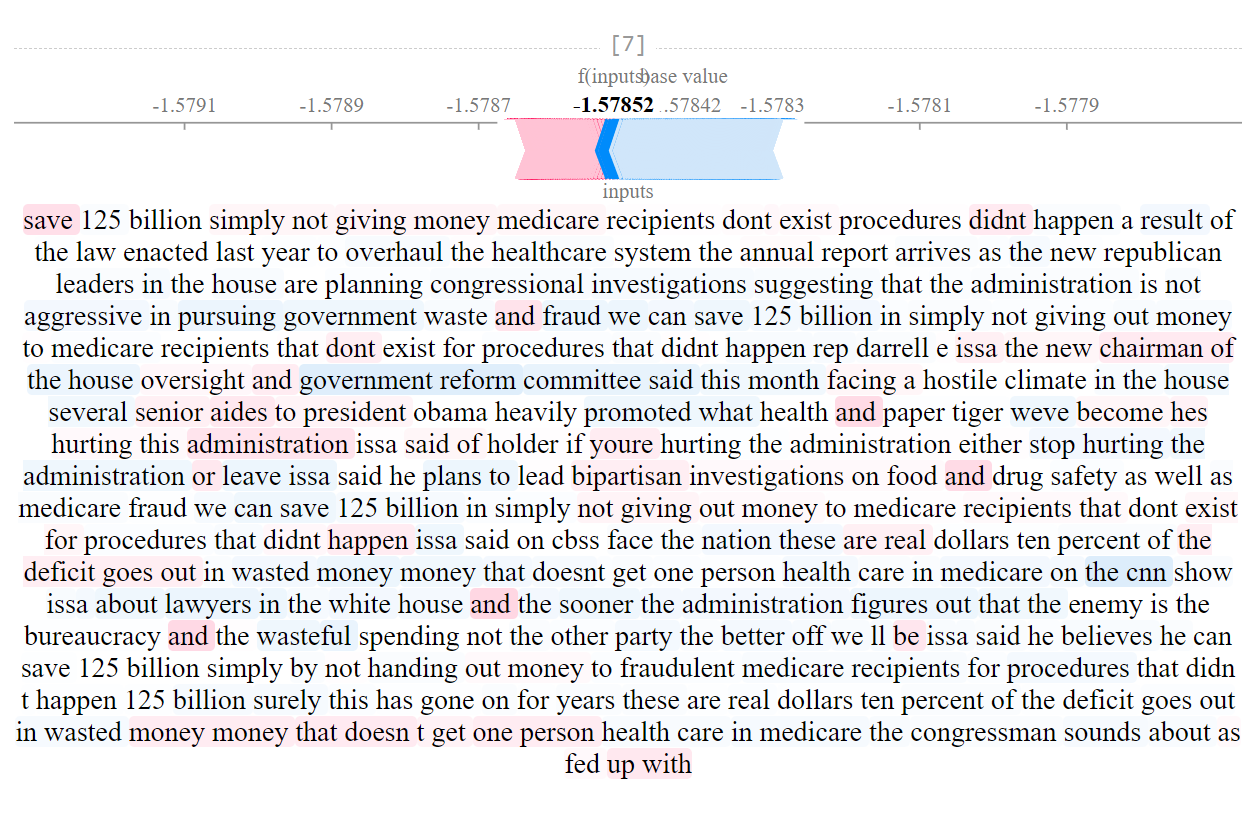
\includegraphics[width=\linewidth]{figs/all_F/bert-l-c.png}
        \caption{{BERT}\textsubscript{L, C}}
    \end{subfigure}


% \end{figure}
% \begin{figure}[h]\ContinuedFloat
%     \captionsetup[subfigure]{justification=Centering}

    % DistilBERT BASE (CASED / CASED MULTILINGUAL)
    \begin{subfigure}[t]{0.4\textwidth}
        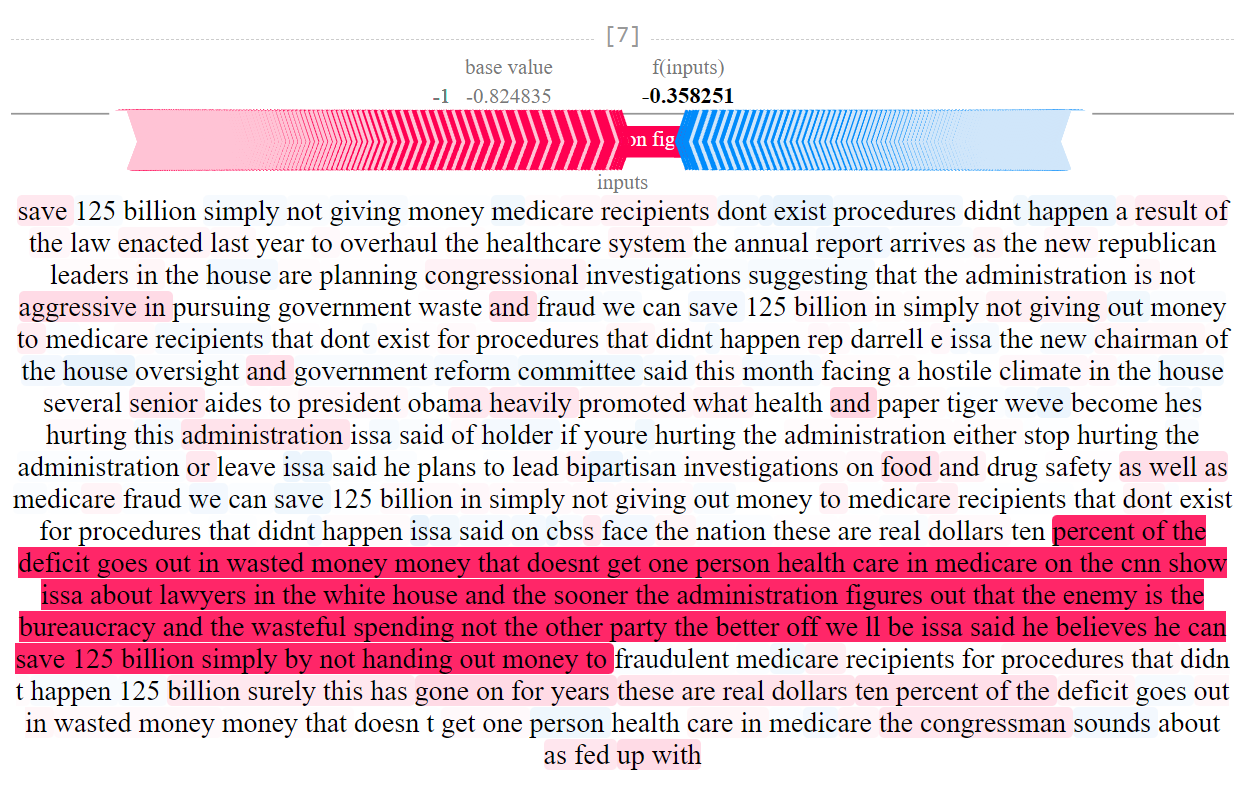
\includegraphics[width=\textwidth]{figs/all_F/distil-b-c.png}
        \caption{{DistilBERT}\textsubscript{B, C}}
    \end{subfigure}
    \hspace{\fill} % maximize horizontal separation
    \begin{subfigure}[t]{0.4\textwidth}
        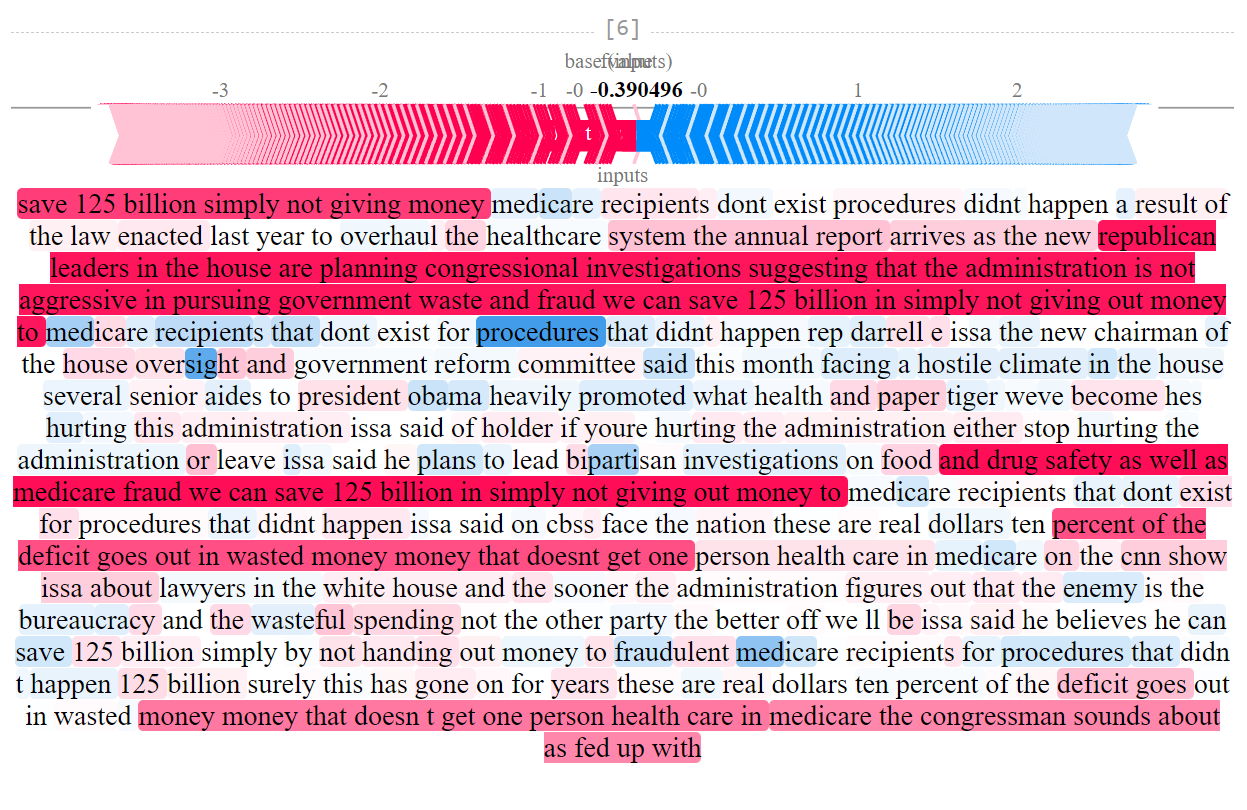
\includegraphics[width=\linewidth]{figs/all_F/bert-b-ml-c.png}
        \caption{{DistilBERT}\textsubscript{B, C, ML}}
    \end{subfigure}


\end{figure}
\begin{figure}[ht]\ContinuedFloat
    \captionsetup[subfigure]{justification=Centering}

    % RoBERTa (BASE / LARGE)
    \begin{subfigure}[t]{0.4\textwidth}
        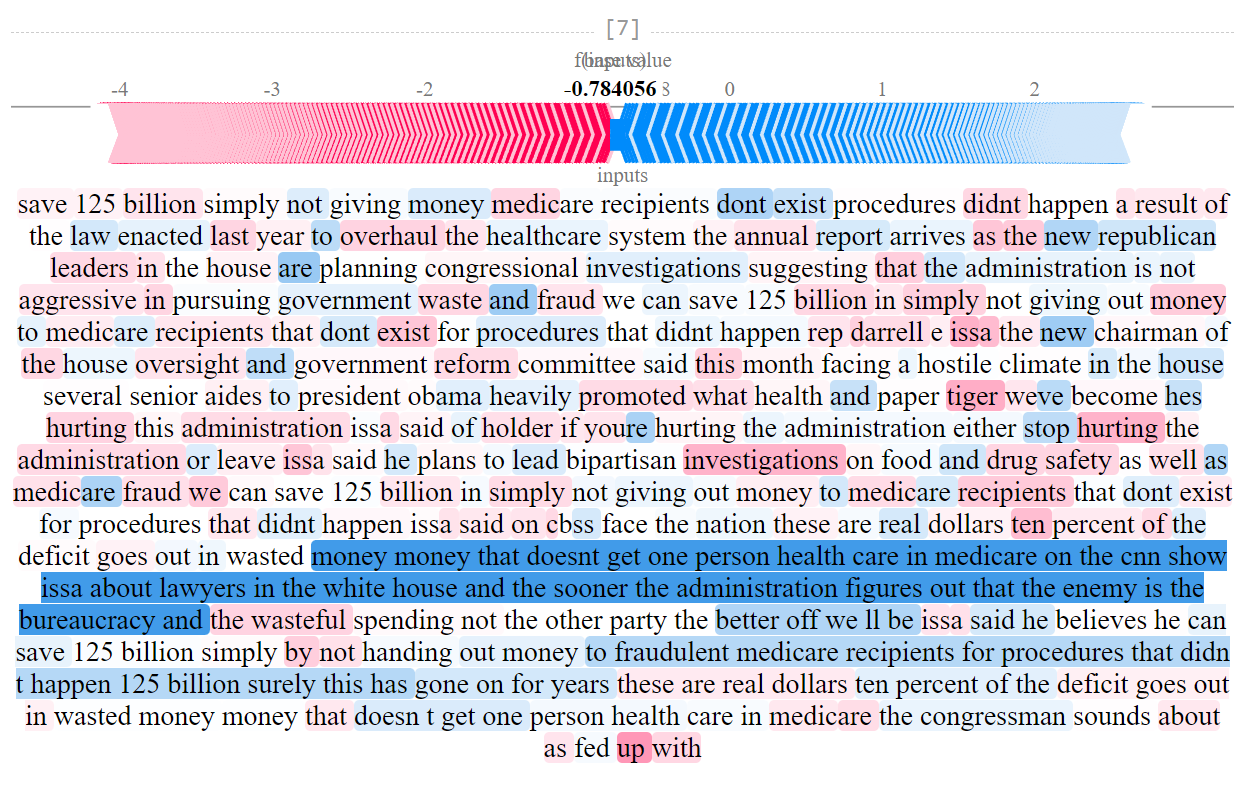
\includegraphics[width=\textwidth]{figs/all_F/roberta-b.png}
        \caption{{RoBERTa}\textsubscript{B}}
    \end{subfigure}
    \hspace{\fill} % maximize horizontal separation
    \begin{subfigure}[t]{0.4\textwidth}
        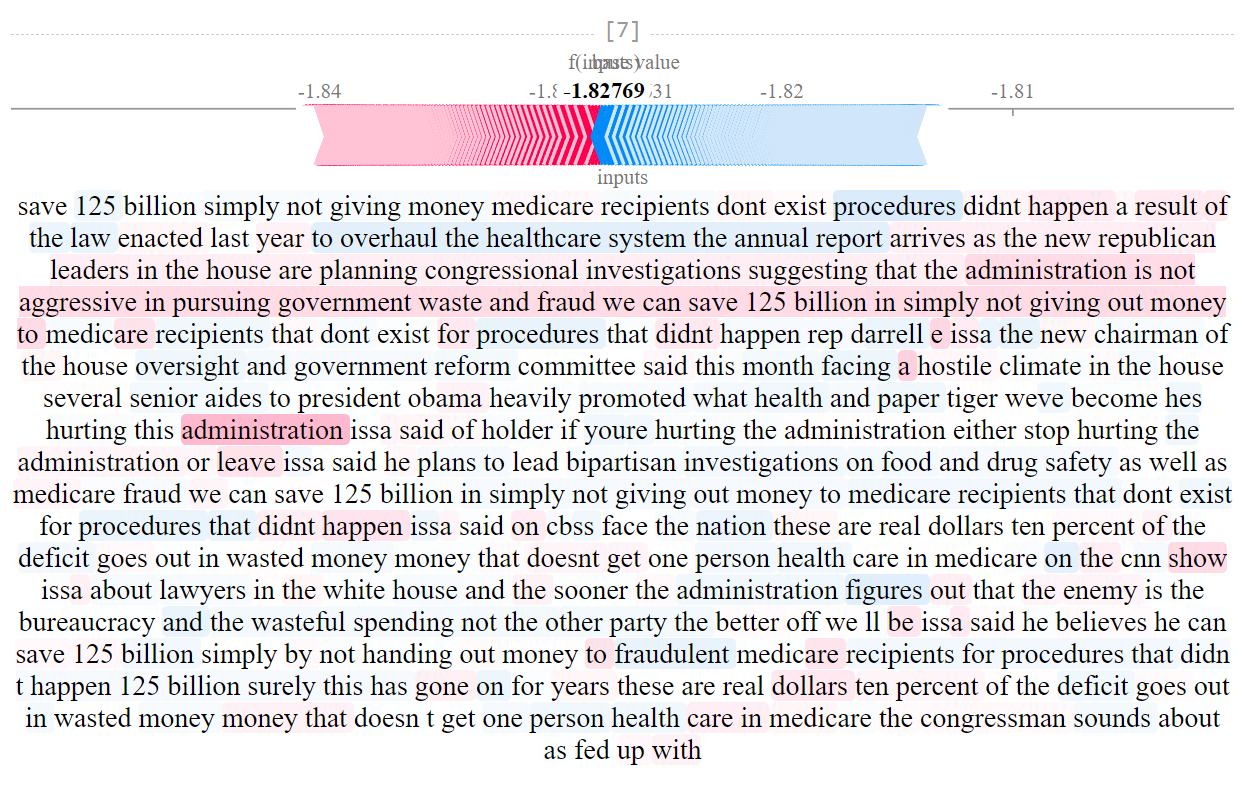
\includegraphics[width=\linewidth]{figs/all_F/roberta-l.png}
        \caption{{RoBERTa}\textsubscript{L}}
    \end{subfigure}


% \end{figure}
% \begin{figure}[h]\ContinuedFloat
%     \captionsetup[subfigure]{justification=Centering}

    % DeBERTa (BASE / LARGE)
    % \bigskip % more vertical separation
    \begin{subfigure}[t]{0.4\textwidth}
        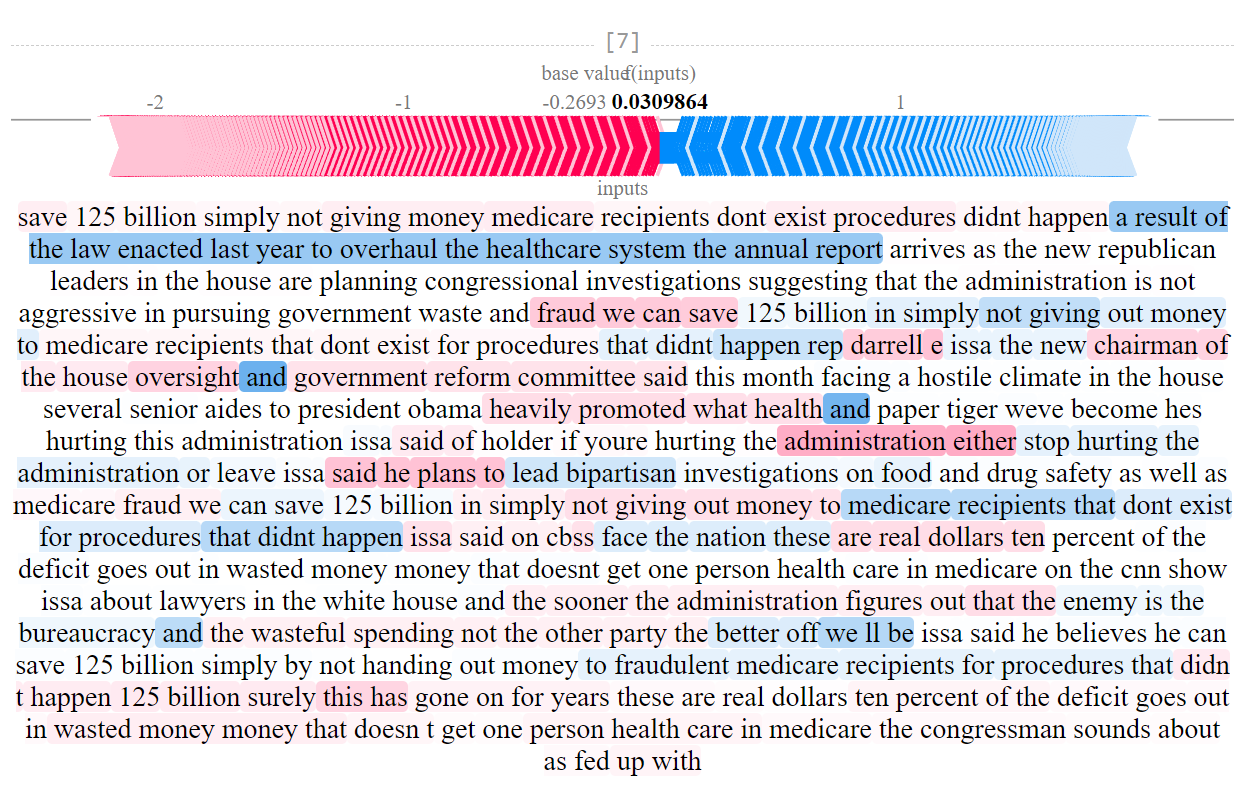
\includegraphics[width=\textwidth]{figs/all_F/deberta-b.png}
        \caption{{DeBERTa}\textsubscript{B}}
    \end{subfigure}
    \hspace{\fill} % maximize horizontal separation
    \begin{subfigure}[t]{0.4\textwidth}
        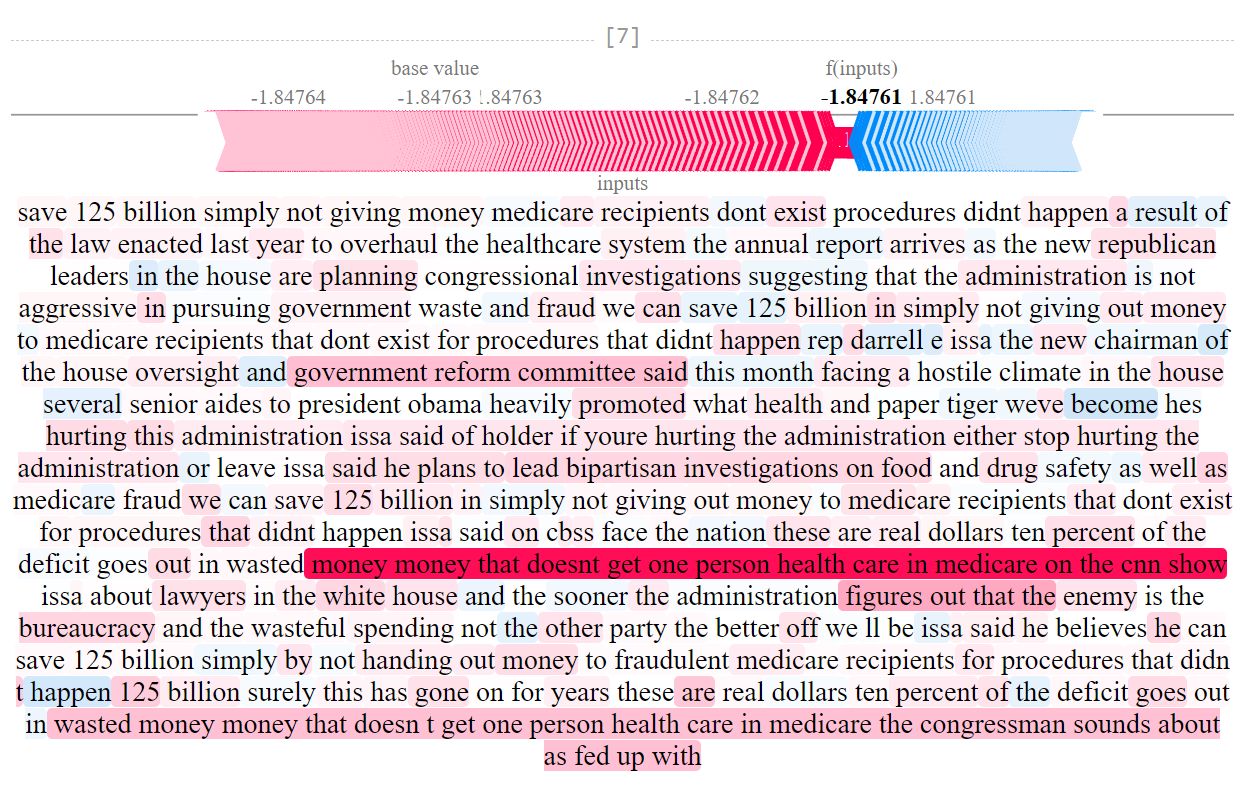
\includegraphics[width=\linewidth]{figs/all_F/deberta-l.png}
        \caption{{DeBERTa}\textsubscript{L}}
    \end{subfigure}    
    
    \caption{Valores Shapley de cada modelo. Los subíndices utilizados para cada modelo $M$ indican respectivamente $M_{\text{B}}$: BASE; $M_{\text{L}}$: LARGE; $M_{C}$: CASED; $M_{\text{U}}$: UNCASED; $M_{\text{ML}}$: MULTILINGUAL.}
\end{figure}


\clearpage
\subsection{News}
\label{fig:shap-news-annex}

\begin{figure}[!h]
    \captionsetup[subfigure]{justification=Centering}
    % BERT BASE (UNCASED / CASED)
    \begin{subfigure}[t]{0.35\textwidth}
        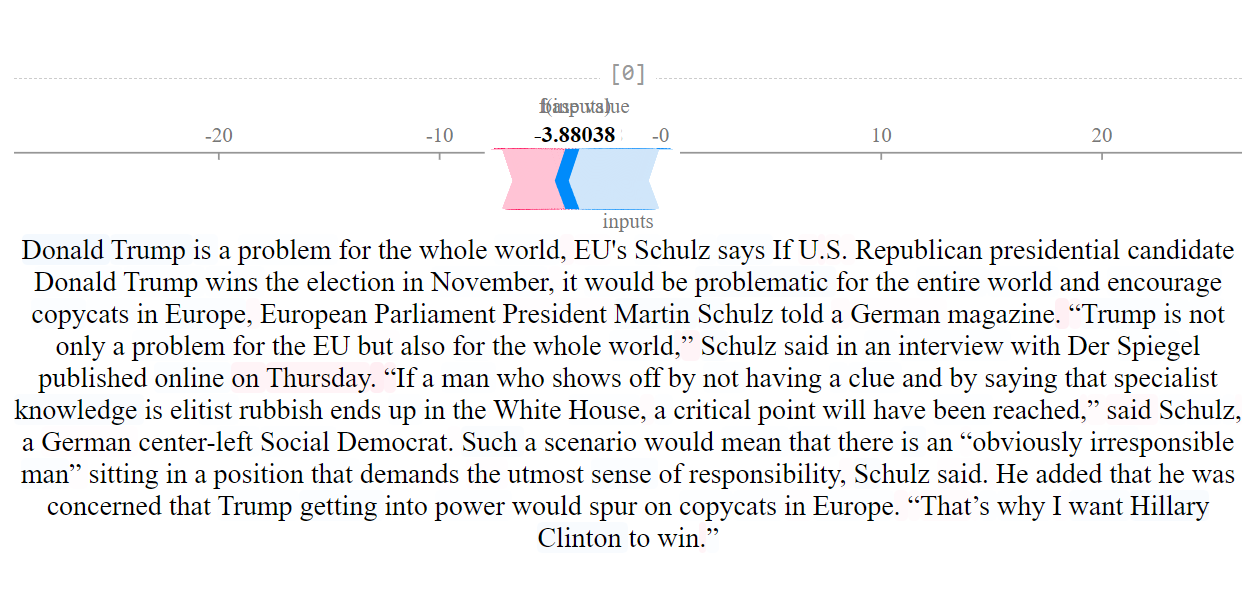
\includegraphics[width=\textwidth]{figs/news_T/bert-b-u.png}
        \caption{{BERT}\textsubscript{B, U}}
    \end{subfigure}
    \hspace{\fill} % maximize horizontal separation
    \begin{subfigure}[t]{0.35\textwidth}
        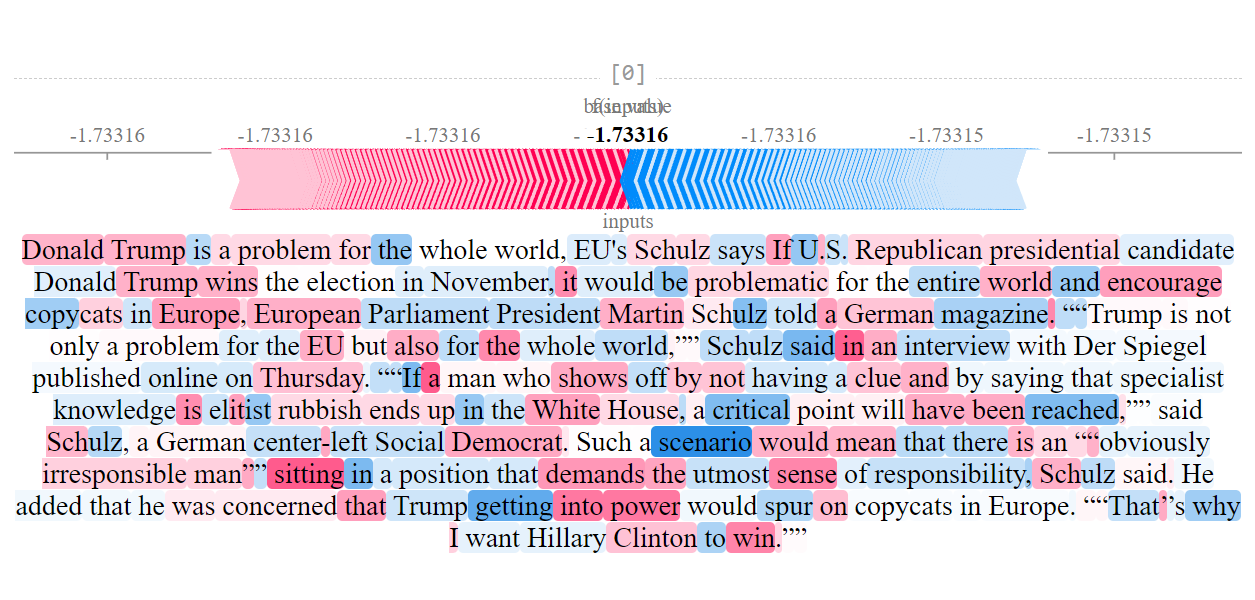
\includegraphics[width=\linewidth]{figs/news_T/bert-b-c.png}
        \caption{{BERT}\textsubscript{B, C}}
    \end{subfigure}


% \end{figure}
% \begin{figure}[h]\ContinuedFloat
%     \captionsetup[subfigure]{justification=Centering}

    % BERT BASE MULTILINGUAL (UNCASED / CASED)
    \begin{subfigure}[t]{0.35\textwidth}
        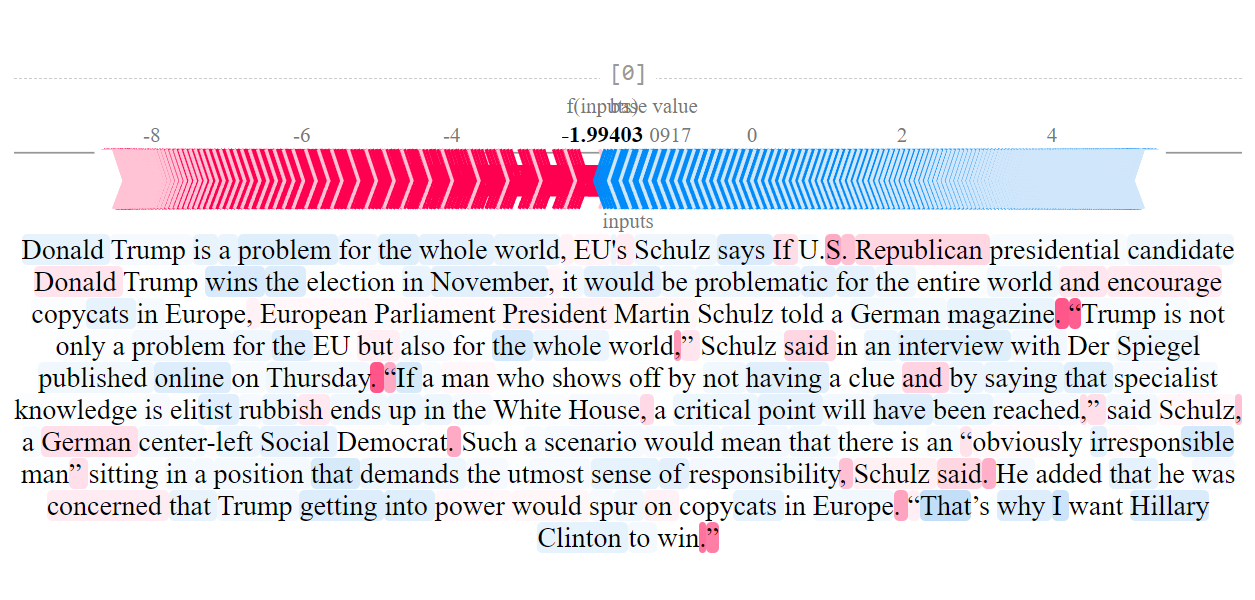
\includegraphics[width=\textwidth]{figs/news_T/bert-b-ml-u.png}
        \caption{{BERT}\textsubscript{B, U, ML}}
    \end{subfigure}
    \hspace{\fill} % maximize horizontal separation
    \begin{subfigure}[t]{0.35\textwidth}
        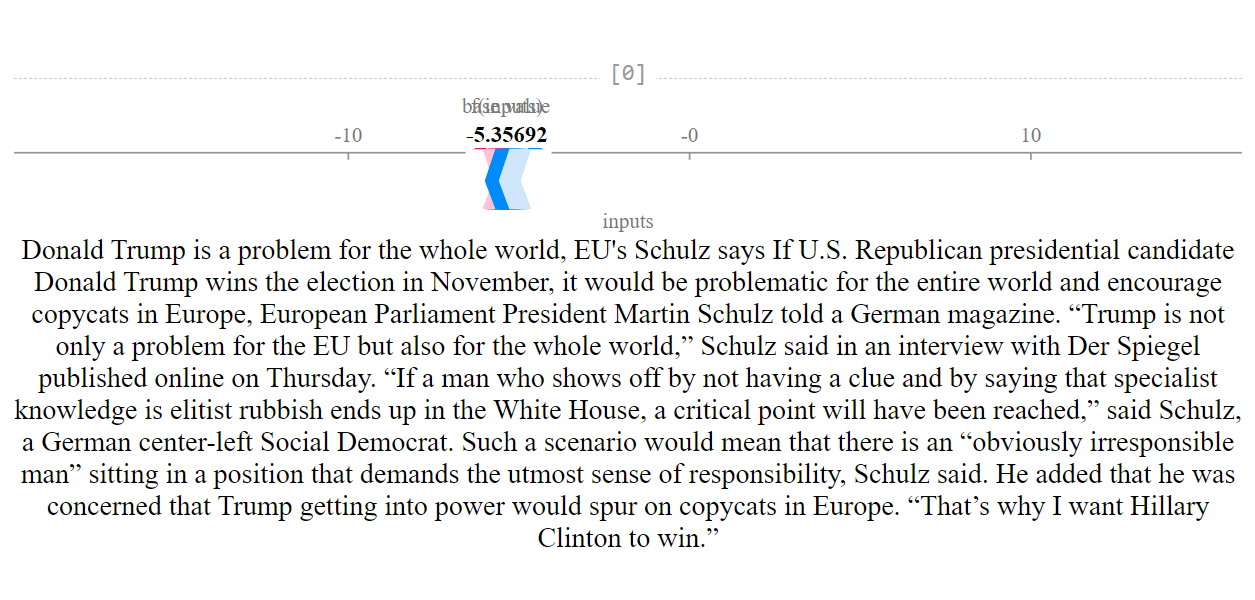
\includegraphics[width=\linewidth]{figs/news_T/bert-b-ml-c.png}
        \caption{{BERT}\textsubscript{B, C, ML}}
    \end{subfigure}


% \end{figure}
% \begin{figure}[h]\ContinuedFloat
%     \captionsetup[subfigure]{justification=Centering}

    % BERT LARGE (UNCASED / CASED)
    \begin{subfigure}[t]{0.35\textwidth}
        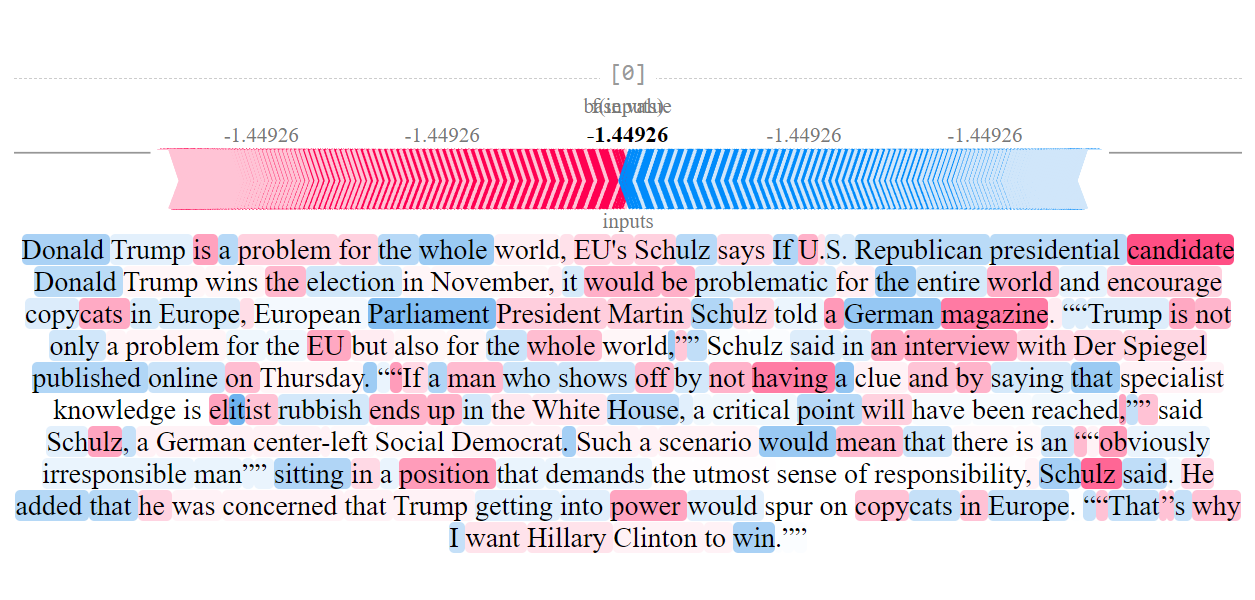
\includegraphics[width=\textwidth]{figs/news_T/bert-l-u.png}
        \caption{{BERT}\textsubscript{L, U}}
    \end{subfigure}
    \hspace{\fill} % maximize horizontal separation
    \begin{subfigure}[t]{0.35\textwidth}
        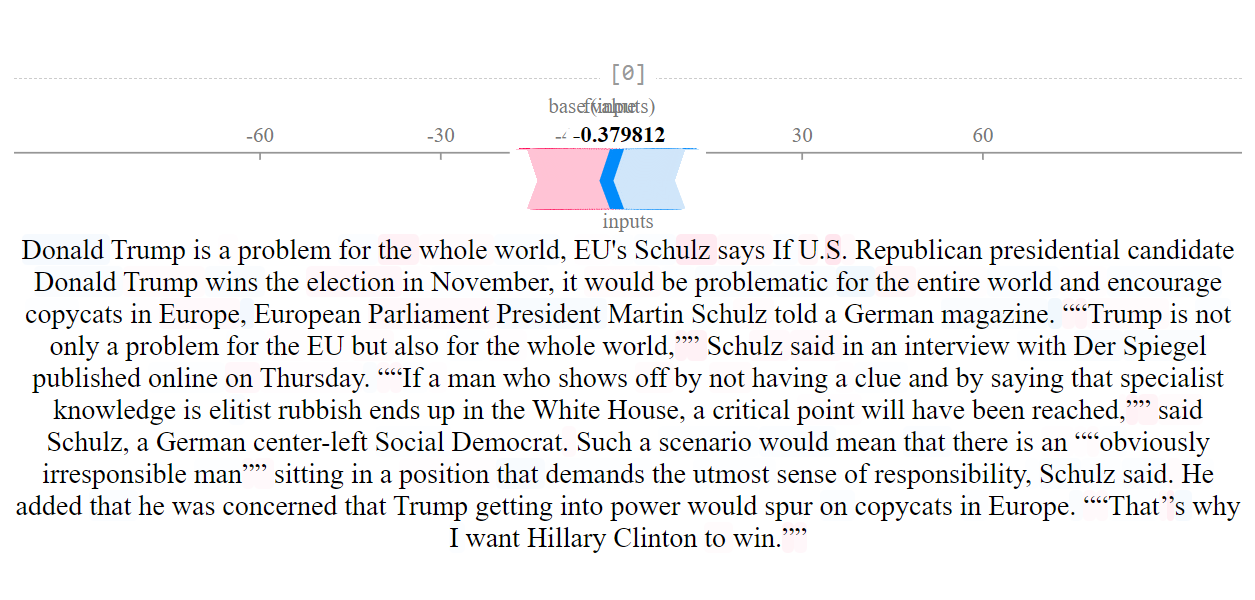
\includegraphics[width=\linewidth]{figs/news_T/bert-l-c.png}
        \caption{{BERT}\textsubscript{L, C}}
    \end{subfigure}


% \end{figure}
% \begin{figure}[h]\ContinuedFloat
%     \captionsetup[subfigure]{justification=Centering}

    % DistilBERT BASE (CASED / CASED MULTILINGUAL)
    \begin{subfigure}[t]{0.35\textwidth}
        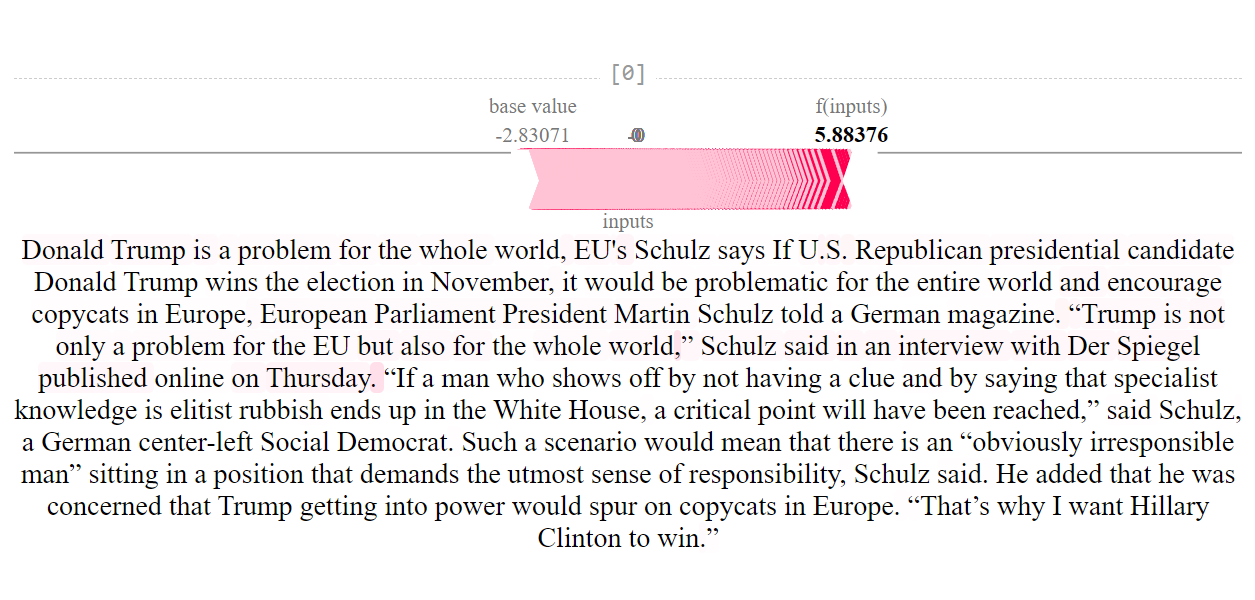
\includegraphics[width=\textwidth]{figs/news_T/distil-b-c.png}
        \caption{{DistilBERT}\textsubscript{B, C}}
    \end{subfigure}
    \hspace{\fill} % maximize horizontal separation
    \begin{subfigure}[t]{0.35\textwidth}
        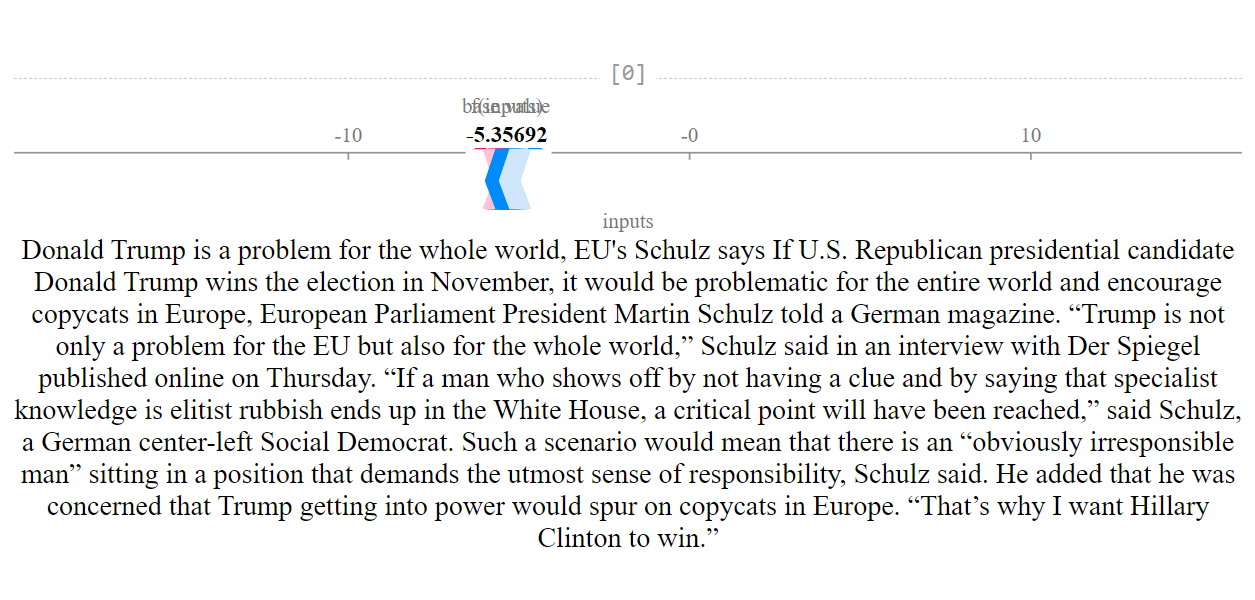
\includegraphics[width=\linewidth]{figs/news_T/bert-b-ml-c.png}
        \caption{{DistilBERT}\textsubscript{B, C, ML}}
    \end{subfigure}


% \end{figure}
% \begin{figure}[!ht]\ContinuedFloat
%     \captionsetup[subfigure]{justification=Centering}

    % RoBERTa (BASE / LARGE)
    \begin{subfigure}[t]{0.35\textwidth}
        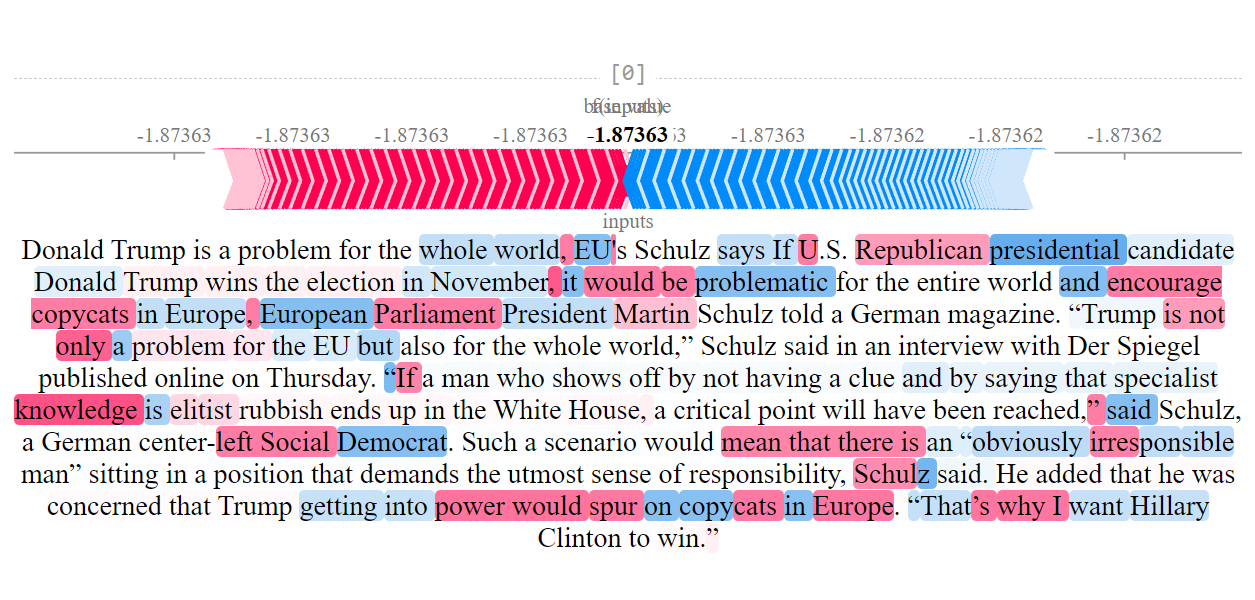
\includegraphics[width=\textwidth]{figs/news_T/roberta-b.png}
        \caption{{RoBERTa}\textsubscript{B}}
    \end{subfigure}
    \hspace{\fill} % maximize horizontal separation
    \begin{subfigure}[t]{0.35\textwidth}
        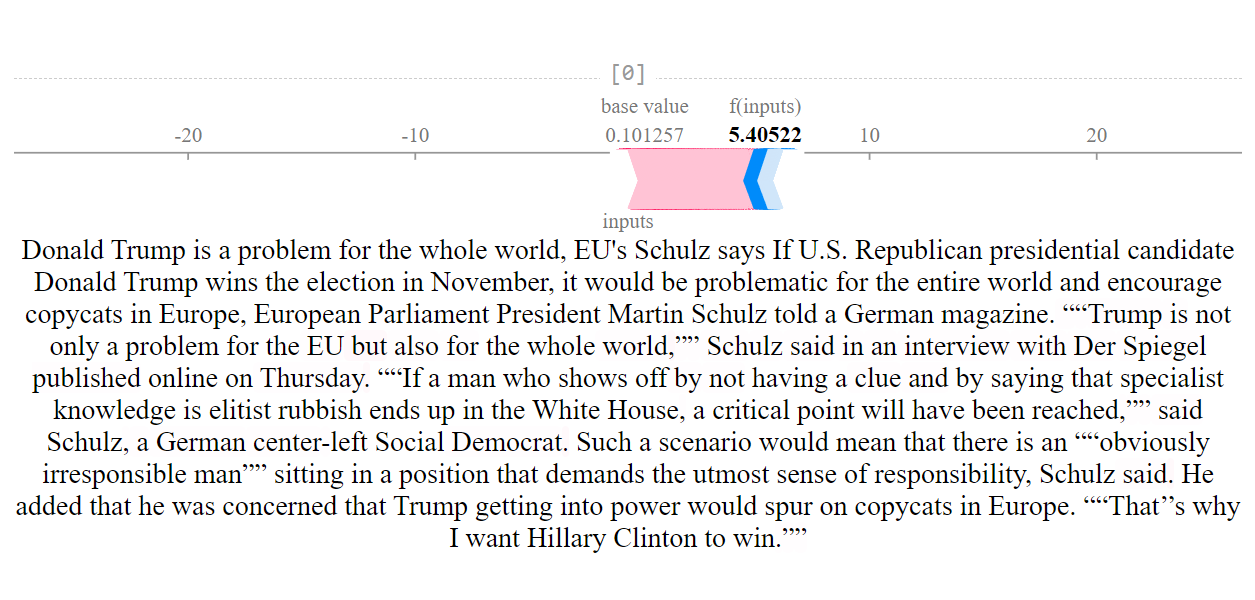
\includegraphics[width=\linewidth]{figs/news_T/roberta-l.png}
        \caption{{RoBERTa}\textsubscript{L}}
    \end{subfigure}


% \end{figure}
% \begin{figure}[h]\ContinuedFloat
%     \captionsetup[subfigure]{justification=Centering}

    % DeBERTa (BASE / LARGE)
    % \bigskip % more vertical separation
    \begin{subfigure}[t]{0.35\textwidth}
        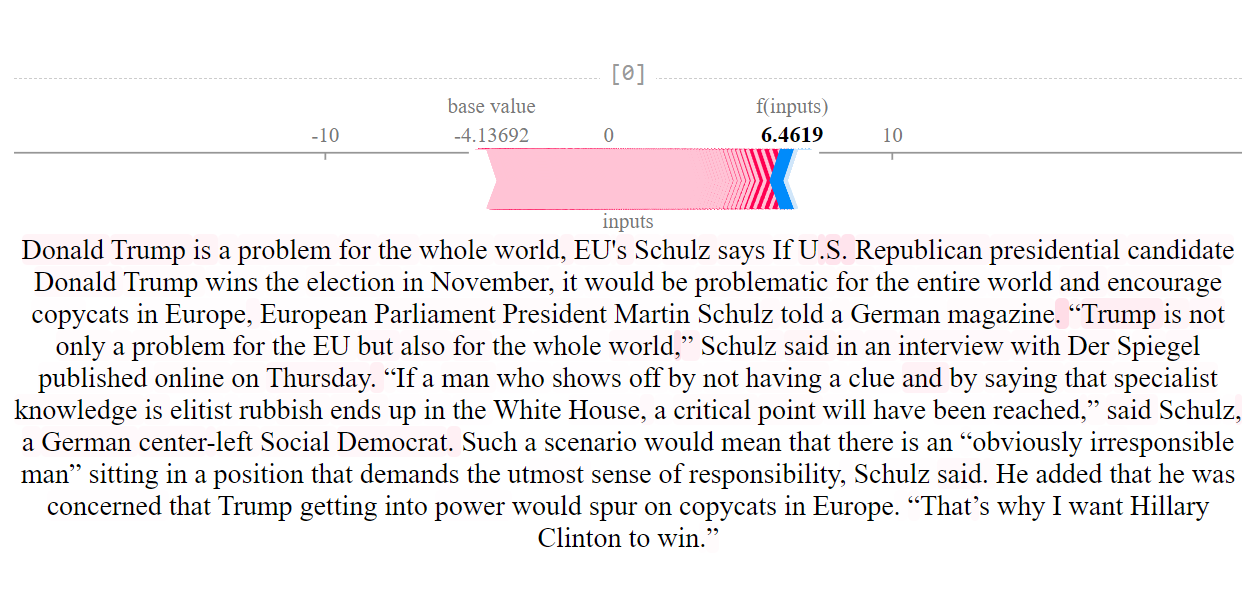
\includegraphics[width=\textwidth]{figs/news_T/deberta-b.png}
        \caption{{DeBERTa}\textsubscript{B}}
    \end{subfigure}
    \hspace{\fill} % maximize horizontal separation
    \begin{subfigure}[t]{0.35\textwidth}
        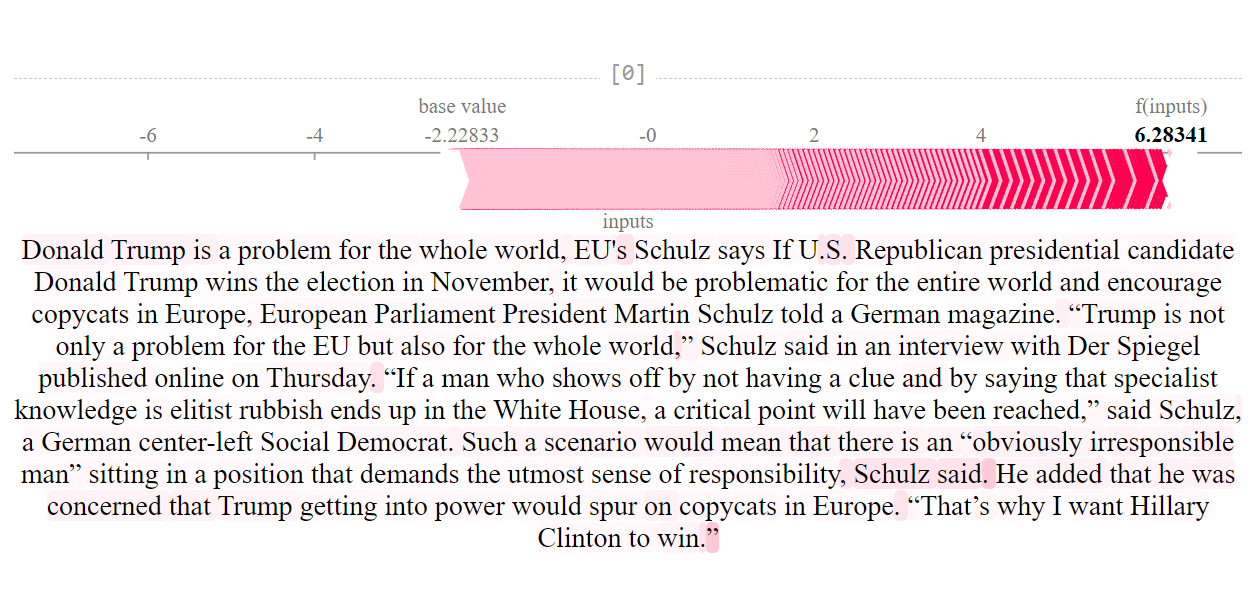
\includegraphics[width=\linewidth]{figs/news_T/deberta-l.png}
        \caption{{DeBERTa}\textsubscript{L}}
    \end{subfigure}    
    
    \caption{Valores Shapley de cada modelo. Los subíndices utilizados para cada modelo $M$ indican respectivamente $M_{\text{B}}$: BASE; $M_{\text{L}}$: LARGE; $M_{C}$: CASED; $M_{\text{U}}$: UNCASED; $M_{\text{ML}}$: MULTILINGUAL.}
\end{figure}

  